\documentclass[11pt,a4paper]{article}
\usepackage[utf8]{inputenc}
\usepackage[T1]{fontenc}
\usepackage[polish]{babel}
\usepackage{lmodern}
\usepackage[margin=2.2cm]{geometry}
\usepackage{graphicx}
\usepackage{booktabs}
\usepackage{longtable}
\usepackage{array}
\usepackage{xcolor}
\usepackage{listings}
\usepackage{caption}
\usepackage{float}
\usepackage{needspace}
\usepackage[hidelinks]{hyperref}

\graphicspath{{img/}{../../llm_judge/results/input/}}
\setlength{\parindent}{0pt}
\setlength{\parskip}{0.5em}
\setlength{\emergencystretch}{3em}

\definecolor{codebg}{RGB}{246,246,246}
\lstset{
  basicstyle=\ttfamily\footnotesize, backgroundcolor=\color{codebg}, frame=single,
  rulecolor=\color{gray!40}, breaklines=true, columns=fullflexible, keepspaces=true,
  showstringspaces=false, keywordstyle=\color{blue!60!black}\bfseries,
  commentstyle=\color{green!40!black}\itshape, stringstyle=\color{red!50!black},
  literate={ą}{{\k{a}}}1 {ć}{{\'c}}1 {ę}{{\k{e}}}1 {ł}{{\l{}}}1 {ń}{{\'n}}1 {ó}{{\'o}}1
           {ś}{{\'s}}1 {ź}{{\'z}}1 {ż}{{\.z}}1 {Ą}{{\k{A}}}1 {Ć}{{\'C}}1 {Ę}{{\k{E}}}1
           {Ł}{{\L{}}}1 {Ń}{{\'N}}1 {Ó}{{\'O}}1 {Ś}{{\'S}}1 {Ź}{{\'Z}}1 {Ż}{{\.Z}}1
           {–}{{--}}1 {≥}{{$\geq$}}1 {×}{{$\times$}}1
}

\begin{document}

% ------------------------------------------------------------------ strona tytułowa
\begin{titlepage}
\centering
{\large Politechnika Wrocławska\par}
\vspace{0.5cm}
{\large Testowanie i jakość oprogramowania (04TIN2-25S302O05245G)\par}
\vspace{3cm}
{\Huge\bfseries Projekt 1: Selenium\par}
\vspace{0.6cm}
{\LARGE Strategia testów i kampania testowa aplikacji Gitea 28.3.0\par}
\vspace{0.6cm}
{\large Raport z testów\par}
\vfill
{\large
\begin{tabular}{l}
\textbf{Zespół:} \\
{Bartosz Olszewski, 294756} \\
{Konrad Mauersberg, 263734} \\
{Adam Ślusarski, 273144} \\
{Maciej Ostojewski, 273190} \\
{Aleksandra Czaińska, 273155} \\[1em]
\textbf{Prowadzący:} Michał Kucharzak \\
\textbf{Termin oddania:} 6.12.2026
\end{tabular}\par}
\vspace{2cm}
{\large Wrocław, rok akademicki 2026/2027\par}
\end{titlepage}

\tableofcontents
\newpage

% ------------------------------------------------------------------ 1
\section{Wprowadzenie i cel projektu}

\subsection{Kontekst i przedmiot testów}
\textbf{Przedmiotem testów} jest \textbf{Gitea 28.3.0} -- otwartoźródłowa (licencja MIT),
samodzielnie hostowana platforma do współpracy nad kodem: repozytoria Git, zgłoszenia (issues),
pull requesty, wiki, zarządzanie uprawnieniami oraz pełne REST API. Aplikacja jest napisana
w Go, ma warstwę webową (szablony + komponenty Vue) i bazę danych, a więc zawiera rozbudowaną
logikę aplikacyjną, a nie tylko statyczne strony. Gitea jest szeroko wykorzystywana przez firmy,
uczelnie i projekty open source jako lekka alternatywa dla GitHub/GitLab, dlatego jej poprawność,
bezpieczeństwo kontroli dostępu i użyteczność mają realne znaczenie dla użytkowników.

Wersja jest przypięta do obrazu \texttt{gitea/gitea:28.3.0} (repozytorium źródłowe:
\url{https://github.com/go-gitea/gitea}), uruchamianego lokalnie przez Docker Compose
(baza SQLite). Dzięki temu \textbf{środowisko testowe} jest powtarzalne lokalnie i w CI.

\subsection{Cel projektu}
Celem projektu jest opracowanie \textbf{strategii testów} oraz realizacja kampanii testowej:
analiza produktu, projekt i automatyzacja przypadków testowych funkcjonalnych
i niefunkcjonalnych, ich wykonanie, ocena UI/UX metodą \emph{LLM-as-a-Judge} oraz
raportowanie wyników zgodnie z nomenklaturą ISTQB CTFL 4.0.

\subsection{Cele testowania}
\begin{itemize}
  \item weryfikacja, czy funkcje o priorytecie \emph{Must} i \emph{Should} działają zgodnie
        z oczekiwaniami (podstawą testów jest dokumentacja Gitea i specyfikacja REST API),
  \item wykrycie defektów w obszarach o najwyższym ryzyku produktowym: uwierzytelnianie,
        kontrola dostępu do repozytoriów prywatnych, przepływ issue/pull request,
  \item ocena wybranych charakterystyk jakości wg ISO/IEC 25010: wydajności, bezpieczeństwa,
        zdolności do interakcji (dostępności) i kompatybilności,
  \item dostarczenie informacji interesariuszom (raport, rejestr defektów) i zbudowanie
        powtarzalnego zestawu testów regresji uruchamianego w CI.
\end{itemize}

\subsection{Zakres prac}
\textbf{W zakresie:} funkcje F01--F10 i F12 (zob. rozdz.~\ref{sec:analiza}); testowanie systemowe
przez interfejs przeglądarki (Selenium WebDriver) i REST API; testy niefunkcjonalne;
LLM-as-a-Judge dla 4 widoków; pipeline CI w GitHub Actions.

\textbf{Poza zakresem:} Gitea Actions (F14), organizacje i wiki (F11, F13 -- świadomie
niepokryte, ryzyko rezydualne), operacje Git przez SSH/HTTP (klient \texttt{git}),
migracje danych, testy pielęgnowalności kodu źródłowego Gitei, testy na urządzeniach mobilnych.

\subsection{Podejście (strategia testów)}
Zastosowano \textbf{testowanie oparte na ryzyku}: priorytet przypadku wynika z priorytetu
MoSCoW funkcji. Przypadki zaprojektowano technikami czarnoskrzynkowymi (podział na klasy
równoważności, analiza wartości brzegowych, tablica decyzyjna, testowanie przejść między
stanami), technikami opartymi na doświadczeniu (zgadywanie błędów, listy kontrolne) oraz
testowaniem opartym na kryteriach akceptacji. Wszystkie testy są na \textbf{poziomie testów
systemowych}; stan systemu przygotowywany jest przez API (szybkie i stabilne warunki wstępne),
a weryfikacja odbywa się w UI i dodatkowo przez API (podwójna wyrocznia testowa).
\textbf{Kryteria wyjścia:} 100\% przypadków wykonanych, wszystkie przypadki o priorytecie
wysokim zaliczone lub z zarejestrowanym defektem, brak otwartych defektów krytycznych
w funkcjach \emph{Must}.

% ------------------------------------------------------------------ 2
\section{Analiza produktu}\label{sec:analiza}
Funkcje zidentyfikowano na podstawie dokumentacji, interfejsu aplikacji i specyfikacji
REST API (\texttt{/api/swagger}). Priorytety nadano metodą \textbf{MoSCoW}
(\emph{Must have}, \emph{Should have}, \emph{Could have}, \emph{Won't have}).

Priorytet określa ważność funkcji dla użytkownika i wynikające z niej ryzyko produktowe,

które wyznacza intensywność testowania (testowanie oparte na ryzyku).

{\small
\begin{longtable}{p{0.188\linewidth}p{0.188\linewidth}p{0.188\linewidth}p{0.188\linewidth}p{0.188\linewidth}}
\toprule
\textbf{ID} & \textbf{Funkcja} & \textbf{Opis} & \textbf{MoSCoW} & \textbf{Uzasadnienie} \\
\midrule
\endhead
F01 & Rejestracja konta & Założenie konta przez formularz \texttt{/user/sign\_up} z walidacją nazwy, e-maila i hasła (min. 8 znaków). & Must & Wejście każdego nowego użytkownika do systemu. \\
F02 & Logowanie i wylogowanie & Uwierzytelnienie nazwą/e-mailem i hasłem, sesja w ciasteczku, wylogowanie z menu użytkownika. & Must & Warunek wstępny niemal wszystkich pozostałych funkcji. \\
F03 & Zarządzanie repozytoriami & Tworzenie (publiczne/prywatne, inicjalizacja README), edycja ustawień i usuwanie repozytoriów. & Must & Podstawowy obiekt domeny aplikacji. \\
F04 & Przeglądanie kodu i historii & Lista plików, podgląd README, historia commitów, gałęzie. & Must & Główny sposób korzystania z repozytorium. \\
F05 & Zgłoszenia (issues) & Tworzenie, komentowanie, zamykanie i ponowne otwieranie zgłoszeń. & Must & Kluczowy proces śledzenia błędów i zadań. \\
F06 & Pull requesty & Porównanie gałęzi, utworzenie PR, przegląd zmian, merge. & Must & Rdzeń współpracy nad kodem. \\
F07 & Kontrola dostępu & Widoczność repo prywatnych, kolaboratorzy z uprawnieniami, ochrona zasobów przed anonimami. & Must & Poufność danych – naruszenie ma wysoki wpływ. \\
F08 & Edytor plików w przeglądarce & Edycja pliku w UI i commit bezpośrednio do gałęzi lub nowej gałęzi. & Should & Wygodne, ale istnieje alternatywa (klient git). \\
F09 & Etykiety i kamienie milowe & Kategoryzacja zgłoszeń etykietami, grupowanie w milestone z licznikiem postępu. & Should & Organizacja pracy zespołu. \\
F10 & Wyszukiwanie & Wyszukiwanie repozytoriów, użytkowników i zgłoszeń (Explore). & Should & Istotne przy dużej liczbie repozytoriów. \\
F11 & Organizacje i zespoły & Grupowanie repo w organizacjach, zespoły z uprawnieniami. & Could & Potrzebne większym zespołom; poza krytyczną ścieżką. \\
F12 & Profil i tokeny API & Ustawienia konta, tokeny dostępu do REST API z zakresami (scopes). & Could & Wykorzystywane przez integracje i automatyzację. \\
F13 & Wiki repozytorium & Strony dokumentacji przy repozytorium. & Could & Funkcja dodatkowa. \\
F14 & Gitea Actions (CI) & Wbudowany system CI kompatybilny z GitHub Actions. & Won't & Poza zakresem – wymaga runnerów, osobny przedmiot testów. \\
\bottomrule
\end{longtable}
}
Podsumowanie: 7 $\times$ Must, 3 $\times$ Should, 3 $\times$ Could, 1 $\times$ Won't.

Funkcje Must są pokryte przypadkami funkcjonalnymi na poziomie UI i/lub API oraz testami

niefunkcjonalnymi; F11 i F13 świadomie nie są pokryte (ryzyko rezydualne, zob. raport §8).



% ------------------------------------------------------------------ 3
\section{Macierz śledzenia}
Macierz śledzenia przedstawia dwukierunkowe powiązanie między funkcjami (elementami
podstawy testów) a przypadkami testowymi. W kodzie powiązanie jest utrzymywane markerami
\texttt{@pytest.mark.tc("TC-...")} i \texttt{@pytest.mark.feature("F..")}, więc każdy wynik
wykonania można przypisać do funkcji.

\needspace{8\baselineskip}\paragraph{Macierz śledzenia (funkcje $\leftrightarrow$ przypadki testowe)}
{\scriptsize\setlength{\tabcolsep}{3pt}
\begin{longtable}{>{\raggedright\arraybackslash}p{\dimexpr 0.130\linewidth-2\tabcolsep\relax}>{\raggedright\arraybackslash}p{\dimexpr 0.062\linewidth-2\tabcolsep\relax}>{\raggedright\arraybackslash}p{\dimexpr 0.062\linewidth-2\tabcolsep\relax}>{\raggedright\arraybackslash}p{\dimexpr 0.062\linewidth-2\tabcolsep\relax}>{\raggedright\arraybackslash}p{\dimexpr 0.062\linewidth-2\tabcolsep\relax}>{\raggedright\arraybackslash}p{\dimexpr 0.062\linewidth-2\tabcolsep\relax}>{\raggedright\arraybackslash}p{\dimexpr 0.062\linewidth-2\tabcolsep\relax}>{\raggedright\arraybackslash}p{\dimexpr 0.062\linewidth-2\tabcolsep\relax}>{\raggedright\arraybackslash}p{\dimexpr 0.062\linewidth-2\tabcolsep\relax}>{\raggedright\arraybackslash}p{\dimexpr 0.062\linewidth-2\tabcolsep\relax}>{\raggedright\arraybackslash}p{\dimexpr 0.062\linewidth-2\tabcolsep\relax}>{\raggedright\arraybackslash}p{\dimexpr 0.062\linewidth-2\tabcolsep\relax}>{\raggedright\arraybackslash}p{\dimexpr 0.062\linewidth-2\tabcolsep\relax}>{\raggedright\arraybackslash}p{\dimexpr 0.062\linewidth-2\tabcolsep\relax}>{\raggedright\arraybackslash}p{\dimexpr 0.062\linewidth-2\tabcolsep\relax}}
\toprule
\textbf{Przypadek} & \textbf{F01} & \textbf{F02} & \textbf{F03} & \textbf{F04} & \textbf{F05} & \textbf{F06} & \textbf{F07} & \textbf{F08} & \textbf{F09} & \textbf{F10} & \textbf{F11} & \textbf{F12} & \textbf{F13} & \textbf{F14} \\
\midrule
\endhead
TC-F01 & \textbullet &  &  &  &  &  &  &  &  &  &  &  &  &  \\
TC-F02 & \textbullet &  &  &  &  &  &  &  &  &  &  &  &  &  \\
TC-F03 &  & \textbullet &  &  &  &  &  &  &  &  &  &  &  &  \\
TC-F04 &  & \textbullet &  &  &  &  &  &  &  &  &  &  &  &  \\
TC-F05 &  &  & \textbullet & \textbullet &  &  &  &  &  &  &  &  &  &  \\
TC-F06 &  &  & \textbullet &  &  &  &  &  &  &  &  &  &  &  \\
TC-F07 &  &  &  &  & \textbullet &  &  &  & \textbullet &  &  &  &  &  \\
TC-F08 &  &  &  &  & \textbullet &  &  &  &  &  &  &  &  &  \\
TC-F09 &  &  &  & \textbullet &  &  &  & \textbullet &  &  &  &  &  &  \\
TC-F10 &  &  &  &  &  & \textbullet &  &  &  &  &  &  &  &  \\
TC-F11 &  &  &  &  &  &  &  &  &  & \textbullet &  &  &  &  \\
TC-F12 &  & \textbullet &  &  &  &  & \textbullet &  &  &  &  &  &  &  \\
TC-F13 &  &  & \textbullet &  &  &  &  &  &  &  &  &  &  &  \\
TC-F14 &  &  &  &  &  &  & \textbullet &  &  &  &  &  &  &  \\
TC-F15 &  &  &  &  &  &  & \textbullet &  &  &  &  &  &  &  \\
TC-F16 &  &  &  &  & \textbullet &  &  &  & \textbullet &  &  &  &  &  \\
TC-F17 &  &  &  &  &  &  &  &  &  &  &  & \textbullet &  &  \\
TC-NF01 &  &  &  & \textbullet & \textbullet &  &  &  &  & \textbullet &  &  &  &  \\
TC-NF02 &  & \textbullet &  & \textbullet & \textbullet &  &  &  &  & \textbullet &  &  &  &  \\
TC-NF03 & \textbullet & \textbullet &  & \textbullet & \textbullet &  &  &  &  &  &  &  &  &  \\
TC-NF04 &  & \textbullet &  &  &  &  & \textbullet &  &  &  &  &  &  &  \\
TC-NF05 &  & \textbullet & \textbullet &  &  &  &  &  &  &  &  &  &  &  \\
\textbf{Liczba TC} & 3 & 7 & 4 & 5 & 6 & 1 & 4 & 1 & 2 & 3 & 0 & 1 & 0 & 0 \\
\bottomrule
\end{longtable}
}
Priorytety MoSCoW funkcji: F01–F07 Must, F08–F10 Should, F11–F13 Could, F14 Won't.

Pokrycie funkcji: 11/14 (79\%); Must 7/7 (100\%), Should 3/3 (100\%), Could 1/3, Won't 0/1 (poza zakresem).

\needspace{8\baselineskip}\paragraph{Podsumowanie przypadków}
{\small
\begin{longtable}{>{\raggedright\arraybackslash}p{\dimexpr 0.090\linewidth-2\tabcolsep\relax}>{\raggedright\arraybackslash}p{\dimexpr 0.190\linewidth-2\tabcolsep\relax}>{\raggedright\arraybackslash}p{\dimexpr 0.090\linewidth-2\tabcolsep\relax}>{\raggedright\arraybackslash}p{\dimexpr 0.150\linewidth-2\tabcolsep\relax}>{\raggedright\arraybackslash}p{\dimexpr 0.110\linewidth-2\tabcolsep\relax}>{\raggedright\arraybackslash}p{\dimexpr 0.110\linewidth-2\tabcolsep\relax}>{\raggedright\arraybackslash}p{\dimexpr 0.120\linewidth-2\tabcolsep\relax}>{\raggedright\arraybackslash}p{\dimexpr 0.140\linewidth-2\tabcolsep\relax}}
\toprule
\textbf{ID} & \textbf{Tytuł} & \textbf{Priorytet} & \textbf{Technika} & \textbf{Poziom} & \textbf{Funkcje} & \textbf{Automatyzacja} & \textbf{Wynik} \\
\midrule
\endhead
TC-F01 & Rejestracja poprawnymi danymi & Wysoki & Klasy równoważności & Systemowy / UI & F01 & Selenium & Zaliczony \\
TC-F02 & Minimalna długość hasła & Wysoki & Wartości brzegowe & Systemowy / UI & F01 & Selenium & Zaliczony \\
TC-F03 & Logowanie poprawne & Wysoki & Klasy równoważności & Systemowy / UI & F02 & Selenium & Zaliczony \\
TC-F04 & Logowanie z błędnym hasłem & Wysoki & Klasy równoważności & Systemowy / UI & F02 & Selenium & Zaliczony \\
TC-F05 & Repozytorium z README & Wysoki & Klasy równoważności & Systemowy / UI & F03, F04 & Selenium & Zaliczony \\
TC-F06 & Duplikat nazwy repo & Średni & Zgadywanie błędów & Systemowy / UI & F03 & Selenium & Zaliczony \\
TC-F07 & Zgłoszenie z etykietą & Wysoki & Kryteria akceptacji & Systemowy / UI & F05, F09 & Selenium & Zaliczony \\
TC-F08 & Zamknięcie i ponowne otwarcie zgłoszenia & Wysoki & Przejścia między stanami & Systemowy / UI & F05 & Selenium & Zaliczony \\
TC-F09 & Edycja pliku w edytorze & Średni & Kryteria akceptacji & Systemowy / UI & F08, F04 & Selenium & Zaliczony \\
TC-F10 & Pull request i merge & Wysoki & Kryteria akceptacji & Systemowy / UI & F06 & Selenium & Zaliczony \\
TC-F11 & Wyszukiwanie repozytorium & Średni & Klasy równoważności & Systemowy / UI & F10 & Selenium & Zaliczony \\
TC-F12 & Wylogowanie a dostęp do ustawień & Wysoki & Przejścia między stanami & Systemowy / UI & F02, F07 & Selenium & Zaliczony \\
TC-F13 & CRUD repozytorium & Wysoki & Kryteria akceptacji & Systemowy / API & F03 & requests & Zaliczony \\
TC-F14 & Widoczność repo wg roli & Wysoki & Tablica decyzyjna & Systemowy / API & F07 & requests & Zaliczony \\
TC-F15 & Kolaborator & Wysoki & Przejścia między stanami & Systemowy / API & F07 & requests & Zaliczony \\
TC-F16 & Postęp milestone & Średni & Kryteria akceptacji & Systemowy / API & F09, F05 & requests & Zaliczony \\
TC-F17 & Token API & Średni & Klasy równoważności & Systemowy / API & F12 & requests & Zaliczony \\
TC-NF01 & Czas odpowiedzi pod obciążeniem & Wysoki & Test obciążeniowy & Systemowy & F04, F05, F10 & Locust & Zaliczony \\
TC-NF02 & Czas ładowania stron & Średni & Pomiar Navigation Timing & Systemowy / UI & F02, F04, F05, F10 & Selenium & Zaliczony \\
TC-NF03 & WCAG 2.1 AA & Średni & Lista kontrolna (axe) & Systemowy / UI & F01, F02, F04, F05 & Selenium + axe & \textbf{Niezaliczony (DEF-02, xfail)} \\
TC-NF04 & Zabezpieczenia aplikacji & Wysoki & Lista kontrolna (ASVS) & Systemowy & F02, F07 & requests & Zaliczony (DEF-01 xfail) \\
TC-NF05 & Kompatybilność przeglądarek & Średni & Test sparametryzowany & Systemowy / UI & F02, F03 & Selenium & Zaliczony \\
\bottomrule
\end{longtable}
}


% ------------------------------------------------------------------ 4
\section{Przypadki testowe}
Poniżej znajduje się 17 przypadków funkcjonalnych (12 realizowanych przez UI z Selenium,
5 przez REST API) i 5 niefunkcjonalnych (w tym 2 wydajnościowe) w ustalonym szablonie.
Źródło: \texttt{docs/test\_cases.md}.

\subsection{Przypadki funkcjonalne}
\subsubsection{TC-F01 – Rejestracja konta poprawnymi danymi}
{\small
\begin{longtable}{p{\dimexpr 0.270\linewidth-2\tabcolsep\relax}p{\dimexpr 0.730\linewidth-2\tabcolsep\relax}}
\toprule
\textbf{Pole} & \textbf{Wartość} \\
\midrule
\endhead
Priorytet & Wysoki \\
Technika & Podział na klasy równoważności (klasa poprawna: unikalna nazwa, poprawny e-mail, hasło $\geq$ 8 znaków) \\
Typ testu & Funkcjonalny \\
Poziom testu & Testowanie systemowe (UI, Selenium) \\
Warunki wstępne / dane & Rejestracja włączona; nazwa \texttt{reg-<losowy>}, e-mail \texttt{<nazwa>@example.com}, hasło \texttt{Valid123!pass}; użytkownik niezalogowany \\
Powiązane funkcje & F01 \\
\bottomrule
\end{longtable}
}
{\small
\begin{longtable}{p{\dimexpr 0.050\linewidth-2\tabcolsep\relax}p{\dimexpr 0.480\linewidth-2\tabcolsep\relax}p{\dimexpr 0.470\linewidth-2\tabcolsep\relax}}
\toprule
\textbf{\#} & \textbf{Krok} & \textbf{Oczekiwany rezultat} \\
\midrule
\endhead
1 & Otwórz \texttt{/user/sign\_up} & Widoczny formularz z polami: nazwa, e-mail, hasło, powtórz hasło \\
2 & Wypełnij pola danymi testowymi & Pola przyjmują wartości, brak komunikatów walidacji \\
3 & Kliknij „Register Account” & Przekierowanie na stronę główną; w nawigacji awatar z nazwą nowego użytkownika \\
4 & Sprawdź \texttt{GET /api/v1/users/<nazwa>} & HTTP 200 \\
\bottomrule
\end{longtable}
}
Warunki końcowe: konto istnieje i jest aktywne, użytkownik zalogowany; po teście konto usunięte przez administratora.

\subsubsection{TC-F02 – Walidacja minimalnej długości hasła przy rejestracji}
{\small
\begin{longtable}{p{\dimexpr 0.270\linewidth-2\tabcolsep\relax}p{\dimexpr 0.730\linewidth-2\tabcolsep\relax}}
\toprule
\textbf{Pole} & \textbf{Wartość} \\
\midrule
\endhead
Priorytet & Wysoki \\
Technika & Analiza wartości brzegowych (dwupunktowa: 7 i 8 znaków; granica \texttt{MIN\_PASSWORD\_LENGTH = 8}) \\
Typ testu & Funkcjonalny \\
Poziom testu & Testowanie systemowe (UI, Selenium) \\
Warunki wstępne / dane & Użytkownik niezalogowany; hasło \texttt{Ab1!Ab1} (7 zn.) oraz \texttt{Ab1!Ab1!} (8 zn.) \\
Powiązane funkcje & F01 \\
\bottomrule
\end{longtable}
}
{\small
\begin{longtable}{p{\dimexpr 0.050\linewidth-2\tabcolsep\relax}p{\dimexpr 0.480\linewidth-2\tabcolsep\relax}p{\dimexpr 0.470\linewidth-2\tabcolsep\relax}}
\toprule
\textbf{\#} & \textbf{Krok} & \textbf{Oczekiwany rezultat} \\
\midrule
\endhead
1 & Otwórz \texttt{/user/sign\_up}, wypełnij formularz hasłem 7-znakowym, wyślij & Komunikat „Password length cannot be less than 8 characters.”; brak przekierowania \\
2 & Sprawdź \texttt{GET /api/v1/users/<nazwa>} & HTTP 404 – konto nie powstało \\
3 & Powtórz krok 1 z hasłem 8-znakowym (nowa nazwa) & Konto utworzone, użytkownik zalogowany (awatar w nawigacji) \\
\bottomrule
\end{longtable}
}
Warunki końcowe: istnieje wyłącznie konto z hasłem 8-znakowym; usunięte po teście.

\subsubsection{TC-F03 – Logowanie poprawnymi danymi}
{\small
\begin{longtable}{p{\dimexpr 0.270\linewidth-2\tabcolsep\relax}p{\dimexpr 0.730\linewidth-2\tabcolsep\relax}}
\toprule
\textbf{Pole} & \textbf{Wartość} \\
\midrule
\endhead
Priorytet & Wysoki \\
Technika & Podział na klasy równoważności (klasa poprawna) \\
Typ testu & Funkcjonalny \\
Poziom testu & Testowanie systemowe (UI, Selenium) \\
Warunki wstępne / dane & Istnieje aktywny użytkownik testowy; przeglądarka bez sesji \\
Powiązane funkcje & F02 \\
\bottomrule
\end{longtable}
}
{\small
\begin{longtable}{p{\dimexpr 0.050\linewidth-2\tabcolsep\relax}p{\dimexpr 0.480\linewidth-2\tabcolsep\relax}p{\dimexpr 0.470\linewidth-2\tabcolsep\relax}}
\toprule
\textbf{\#} & \textbf{Krok} & \textbf{Oczekiwany rezultat} \\
\midrule
\endhead
1 & Otwórz \texttt{/user/login} & Formularz z polami nazwy i hasła \\
2 & Wpisz poprawną nazwę i hasło, kliknij „Sign In” & Przekierowanie na \texttt{/} \\
3 & Sprawdź nawigację & Awatar z tytułem równym nazwie użytkownika \\
\bottomrule
\end{longtable}
}
Warunki końcowe: aktywna sesja użytkownika testowego.

\subsubsection{TC-F04 – Odrzucenie logowania z błędnym hasłem}
{\small
\begin{longtable}{p{\dimexpr 0.270\linewidth-2\tabcolsep\relax}p{\dimexpr 0.730\linewidth-2\tabcolsep\relax}}
\toprule
\textbf{Pole} & \textbf{Wartość} \\
\midrule
\endhead
Priorytet & Wysoki \\
Technika & Podział na klasy równoważności (klasa niepoprawna: błędne hasło) \\
Typ testu & Funkcjonalny \\
Poziom testu & Testowanie systemowe (UI, Selenium) \\
Warunki wstępne / dane & Istnieje użytkownik testowy; hasło \texttt{wrong-password} \\
Powiązane funkcje & F02 \\
\bottomrule
\end{longtable}
}
{\small
\begin{longtable}{p{\dimexpr 0.050\linewidth-2\tabcolsep\relax}p{\dimexpr 0.480\linewidth-2\tabcolsep\relax}p{\dimexpr 0.470\linewidth-2\tabcolsep\relax}}
\toprule
\textbf{\#} & \textbf{Krok} & \textbf{Oczekiwany rezultat} \\
\midrule
\endhead
1 & Otwórz \texttt{/user/login} & Formularz logowania \\
2 & Wpisz poprawną nazwę i błędne hasło, wyślij & Komunikat „Username or password is incorrect.” \\
3 & Sprawdź URL i nawigację & URL zawiera \texttt{/user/login}; brak awatara (użytkownik niezalogowany) \\
\bottomrule
\end{longtable}
}
Warunki końcowe: brak sesji; konto nie zostało zablokowane.

\subsubsection{TC-F05 – Utworzenie repozytorium z plikiem README}
{\small
\begin{longtable}{p{\dimexpr 0.270\linewidth-2\tabcolsep\relax}p{\dimexpr 0.730\linewidth-2\tabcolsep\relax}}
\toprule
\textbf{Pole} & \textbf{Wartość} \\
\midrule
\endhead
Priorytet & Wysoki \\
Technika & Podział na klasy równoważności (poprawna nazwa, repo publiczne, inicjalizacja włączona) \\
Typ testu & Funkcjonalny \\
Poziom testu & Testowanie systemowe (UI, Selenium + weryfikacja API) \\
Warunki wstępne / dane & Zalogowany użytkownik testowy; nazwa \texttt{ui-repo-<losowy>}, opis „Repo z testu Selenium” \\
Powiązane funkcje & F03, F04 \\
\bottomrule
\end{longtable}
}
{\small
\begin{longtable}{p{\dimexpr 0.050\linewidth-2\tabcolsep\relax}p{\dimexpr 0.480\linewidth-2\tabcolsep\relax}p{\dimexpr 0.470\linewidth-2\tabcolsep\relax}}
\toprule
\textbf{\#} & \textbf{Krok} & \textbf{Oczekiwany rezultat} \\
\midrule
\endhead
1 & Otwórz \texttt{/repo/create} & Formularz nowego repozytorium \\
2 & Podaj nazwę i opis, zaznacz „Initialize Repository”, kliknij „Create Repository” & Przekierowanie na \texttt{/<użytkownik>/<nazwa>} \\
3 & Sprawdź listę plików & Lista zawiera \texttt{README.md} \\
4 & Sprawdź sekcję README & Zawiera nazwę repo i opis \\
5 & \texttt{GET /api/v1/repos/<użytkownik>/<nazwa>} & \texttt{description} = opis, \texttt{private} = false \\
\bottomrule
\end{longtable}
}
Warunki końcowe: repozytorium istnieje z jednym commitem; usunięte po teście.

\subsubsection{TC-F06 – Odrzucenie duplikatu nazwy repozytorium}
{\small
\begin{longtable}{p{\dimexpr 0.270\linewidth-2\tabcolsep\relax}p{\dimexpr 0.730\linewidth-2\tabcolsep\relax}}
\toprule
\textbf{Pole} & \textbf{Wartość} \\
\midrule
\endhead
Priorytet & Średni \\
Technika & Zgadywanie błędów (error guessing) \\
Typ testu & Funkcjonalny \\
Poziom testu & Testowanie systemowe (UI, Selenium) \\
Warunki wstępne / dane & Zalogowany użytkownik; istnieje jego repozytorium o nazwie X (utworzone przez API) \\
Powiązane funkcje & F03 \\
\bottomrule
\end{longtable}
}
{\small
\begin{longtable}{p{\dimexpr 0.050\linewidth-2\tabcolsep\relax}p{\dimexpr 0.480\linewidth-2\tabcolsep\relax}p{\dimexpr 0.470\linewidth-2\tabcolsep\relax}}
\toprule
\textbf{\#} & \textbf{Krok} & \textbf{Oczekiwany rezultat} \\
\midrule
\endhead
1 & Otwórz \texttt{/repo/create}, podaj nazwę X, wyślij & Komunikat „The repository name is already used.” \\
2 & Sprawdź URL & Pozostaje \texttt{/repo/create} \\
3 & \texttt{GET /api/v1/user/repos} & Nazwa X występuje dokładnie raz \\
\bottomrule
\end{longtable}
}
Warunki końcowe: stan repozytoriów użytkownika bez zmian.

\subsubsection{TC-F07 – Utworzenie zgłoszenia z etykietą}
{\small
\begin{longtable}{p{\dimexpr 0.270\linewidth-2\tabcolsep\relax}p{\dimexpr 0.730\linewidth-2\tabcolsep\relax}}
\toprule
\textbf{Pole} & \textbf{Wartość} \\
\midrule
\endhead
Priorytet & Wysoki \\
Technika & Testowanie oparte na kryteriach akceptacji \\
Typ testu & Funkcjonalny \\
Poziom testu & Testowanie systemowe (UI, Selenium + weryfikacja API) \\
Warunki wstępne / dane & Zalogowany właściciel repozytorium; w repo istnieje etykieta \texttt{bug}; tytuł „Błąd logowania-<losowy>” \\
Powiązane funkcje & F05, F09 \\
\bottomrule
\end{longtable}
}
{\small
\begin{longtable}{p{\dimexpr 0.050\linewidth-2\tabcolsep\relax}p{\dimexpr 0.480\linewidth-2\tabcolsep\relax}p{\dimexpr 0.470\linewidth-2\tabcolsep\relax}}
\toprule
\textbf{\#} & \textbf{Krok} & \textbf{Oczekiwany rezultat} \\
\midrule
\endhead
1 & Otwórz \texttt{/<repo>/issues/new} & Formularz z polem tytułu, opisem i panelem bocznym \\
2 & Wpisz tytuł i opis & Wartości widoczne w polach \\
3 & W panelu „Labels” wybierz \texttt{bug}, zamknij listę & Etykieta \texttt{bug} widoczna w panelu \\
4 & Kliknij „Create Issue” & Przekierowanie na \texttt{/<repo>/issues/<n>}; tytuł i etykieta \texttt{bug} widoczne \\
5 & \texttt{GET /api/v1/repos/<repo>/issues/<n>} & \texttt{state} = open, \texttt{labels} = [\texttt{bug}] \\
\bottomrule
\end{longtable}
}
Warunki końcowe: w repo istnieje 1 otwarte zgłoszenie z etykietą \texttt{bug}.

\subsubsection{TC-F08 – Komentarz, zamknięcie i ponowne otwarcie zgłoszenia}
{\small
\begin{longtable}{p{\dimexpr 0.270\linewidth-2\tabcolsep\relax}p{\dimexpr 0.730\linewidth-2\tabcolsep\relax}}
\toprule
\textbf{Pole} & \textbf{Wartość} \\
\midrule
\endhead
Priorytet & Wysoki \\
Technika & Testowanie przejść między stanami (open $\rightarrow$ closed $\rightarrow$ open; przejścia „zamknij z komentarzem”, „otwórz ponownie”) \\
Typ testu & Funkcjonalny \\
Poziom testu & Testowanie systemowe (UI, Selenium + weryfikacja API) \\
Warunki wstępne / dane & Zalogowany właściciel; otwarte zgłoszenie „Do zamknięcia” utworzone przez API \\
Powiązane funkcje & F05 \\
\bottomrule
\end{longtable}
}
{\small
\begin{longtable}{p{\dimexpr 0.050\linewidth-2\tabcolsep\relax}p{\dimexpr 0.480\linewidth-2\tabcolsep\relax}p{\dimexpr 0.470\linewidth-2\tabcolsep\relax}}
\toprule
\textbf{\#} & \textbf{Krok} & \textbf{Oczekiwany rezultat} \\
\midrule
\endhead
1 & Otwórz stronę zgłoszenia & Przycisk statusu „Close Issue” \\
2 & Dodaj komentarz „Potwierdzam błąd” & Komentarz widoczny na osi czasu; stan nadal open \\
3 & Wpisz „Naprawione” i kliknij „Close with Comment” & Stan w API = closed; przycisk zmienia się na „Reopen Issue” \\
4 & Kliknij „Reopen Issue” & Stan w API = open \\
5 & \texttt{GET .../issues/<n>/comments} & Dokładnie 2 komentarze w kolejności: „Potwierdzam błąd”, „Naprawione” \\
\bottomrule
\end{longtable}
}
Warunki końcowe: zgłoszenie otwarte, 2 komentarze, 2 zdarzenia zmiany stanu na osi czasu.

\subsubsection{TC-F09 – Edycja pliku w edytorze przeglądarkowym i commit}
{\small
\begin{longtable}{p{\dimexpr 0.270\linewidth-2\tabcolsep\relax}p{\dimexpr 0.730\linewidth-2\tabcolsep\relax}}
\toprule
\textbf{Pole} & \textbf{Wartość} \\
\midrule
\endhead
Priorytet & Średni \\
Technika & Testowanie oparte na kryteriach akceptacji \\
Typ testu & Funkcjonalny \\
Poziom testu & Testowanie systemowe (UI, Selenium + weryfikacja API) \\
Warunki wstępne / dane & Zalogowany właściciel repo z \texttt{README.md}; nowa treść „Treść zmieniona w edytorze”; opis commita „Aktualizacja README z UI” \\
Powiązane funkcje & F08, F04 \\
\bottomrule
\end{longtable}
}
{\small
\begin{longtable}{p{\dimexpr 0.050\linewidth-2\tabcolsep\relax}p{\dimexpr 0.480\linewidth-2\tabcolsep\relax}p{\dimexpr 0.470\linewidth-2\tabcolsep\relax}}
\toprule
\textbf{\#} & \textbf{Krok} & \textbf{Oczekiwany rezultat} \\
\midrule
\endhead
1 & Otwórz \texttt{/<repo>/\_edit/main/README.md} & Edytor kodu z bieżącą treścią pliku \\
2 & Zaznacz całą treść i zastąp nową & Edytor zawiera wyłącznie nową treść \\
3 & Wpisz opis commita, wybierz „Commit directly”, kliknij „Commit Changes” & Przekierowanie do widoku pliku \texttt{/src/branch/main/...} \\
4 & \texttt{GET .../contents/README.md} & Zdekodowana treść = nowa treść \\
5 & \texttt{GET .../commits?limit=1} & Wiadomość ostatniego commita = podany opis \\
\bottomrule
\end{longtable}
}
Warunki końcowe: gałąź \texttt{main} ma nowy commit ze zmienionym README.

\subsubsection{TC-F10 – Utworzenie i scalenie pull requesta}
{\small
\begin{longtable}{p{\dimexpr 0.270\linewidth-2\tabcolsep\relax}p{\dimexpr 0.730\linewidth-2\tabcolsep\relax}}
\toprule
\textbf{Pole} & \textbf{Wartość} \\
\midrule
\endhead
Priorytet & Wysoki \\
Technika & Testowanie oparte na kryteriach akceptacji (przepływ end-to-end) \\
Typ testu & Funkcjonalny \\
Poziom testu & Testowanie systemowe (UI, Selenium + weryfikacja API) \\
Warunki wstępne / dane & Zalogowany właściciel; gałąź \texttt{feature-x} z plikiem \texttt{feature.txt} (utworzona przez API); tytuł PR „Dodaje feature.txt” \\
Powiązane funkcje & F06 \\
\bottomrule
\end{longtable}
}
{\small
\begin{longtable}{p{\dimexpr 0.050\linewidth-2\tabcolsep\relax}p{\dimexpr 0.480\linewidth-2\tabcolsep\relax}p{\dimexpr 0.470\linewidth-2\tabcolsep\relax}}
\toprule
\textbf{\#} & \textbf{Krok} & \textbf{Oczekiwany rezultat} \\
\midrule
\endhead
1 & Otwórz \texttt{/<repo>/compare/main...feature-x} & Diff z 1 zmienionym plikiem, przycisk „New Pull Request” \\
2 & Kliknij „New Pull Request”, wpisz tytuł, „Create Pull Request” & Przekierowanie na \texttt{/<repo>/pulls/<n>} \\
3 & Kliknij „Create merge commit” i potwierdź & Etykieta stanu „Merged” \\
4 & \texttt{GET .../pulls/<n>} & \texttt{merged} = true \\
5 & \texttt{GET .../contents/feature.txt?ref=main} & HTTP 200 – plik w \texttt{main} \\
\bottomrule
\end{longtable}
}
Warunki końcowe: PR scalony i zamknięty, \texttt{main} zawiera \texttt{feature.txt}.

\subsubsection{TC-F11 – Wyszukiwanie repozytorium po nazwie}
{\small
\begin{longtable}{p{\dimexpr 0.270\linewidth-2\tabcolsep\relax}p{\dimexpr 0.730\linewidth-2\tabcolsep\relax}}
\toprule
\textbf{Pole} & \textbf{Wartość} \\
\midrule
\endhead
Priorytet & Średni \\
Technika & Podział na klasy równoważności (repo pasujące / niepasujące do frazy) \\
Typ testu & Funkcjonalny \\
Poziom testu & Testowanie systemowe (UI, Selenium) \\
Warunki wstępne / dane & Zalogowany użytkownik; repo \texttt{szukaj-<losowy>-app} oraz repo o niepasującej nazwie \\
Powiązane funkcje & F10 \\
\bottomrule
\end{longtable}
}
{\small
\begin{longtable}{p{\dimexpr 0.050\linewidth-2\tabcolsep\relax}p{\dimexpr 0.480\linewidth-2\tabcolsep\relax}p{\dimexpr 0.470\linewidth-2\tabcolsep\relax}}
\toprule
\textbf{\#} & \textbf{Krok} & \textbf{Oczekiwany rezultat} \\
\midrule
\endhead
1 & Otwórz \texttt{/explore/repos} & Pole wyszukiwania i lista repozytoriów \\
2 & Wpisz frazę \texttt{szukaj-<losowy>}, Enter & URL zawiera \texttt{q=} \\
3 & Odczytaj wyniki & Repo pasujące jest na liście, repo niepasujące – nie \\
\bottomrule
\end{longtable}
}
Warunki końcowe: brak zmian danych (oba repo usunięte po teście).

\subsubsection{TC-F12 – Wylogowanie blokuje dostęp do ustawień konta}
{\small
\begin{longtable}{p{\dimexpr 0.270\linewidth-2\tabcolsep\relax}p{\dimexpr 0.730\linewidth-2\tabcolsep\relax}}
\toprule
\textbf{Pole} & \textbf{Wartość} \\
\midrule
\endhead
Priorytet & Wysoki \\
Technika & Testowanie przejść między stanami (zalogowany $\rightarrow$ niezalogowany) \\
Typ testu & Funkcjonalny \\
Poziom testu & Testowanie systemowe (UI, Selenium) \\
Warunki wstępne / dane & Zalogowany użytkownik testowy \\
Powiązane funkcje & F02, F07 \\
\bottomrule
\end{longtable}
}
{\small
\begin{longtable}{p{\dimexpr 0.050\linewidth-2\tabcolsep\relax}p{\dimexpr 0.480\linewidth-2\tabcolsep\relax}p{\dimexpr 0.470\linewidth-2\tabcolsep\relax}}
\toprule
\textbf{\#} & \textbf{Krok} & \textbf{Oczekiwany rezultat} \\
\midrule
\endhead
1 & Otwórz menu awatara, kliknij „Sign Out” & W nawigacji link „Sign In”, brak awatara \\
2 & Otwórz \texttt{/user/settings} & Przekierowanie na \texttt{/user/login?redirect\_to=\%2Fuser\%2Fsettings} \\
\bottomrule
\end{longtable}
}
Warunki końcowe: brak aktywnej sesji.

\subsubsection{TC-F13 – CRUD repozytorium przez REST API}
{\small
\begin{longtable}{p{\dimexpr 0.270\linewidth-2\tabcolsep\relax}p{\dimexpr 0.730\linewidth-2\tabcolsep\relax}}
\toprule
\textbf{Pole} & \textbf{Wartość} \\
\midrule
\endhead
Priorytet & Wysoki \\
Technika & Testowanie oparte na kryteriach akceptacji (cykl życia zasobu) \\
Typ testu & Funkcjonalny \\
Poziom testu & Testowanie systemowe (REST API) \\
Warunki wstępne / dane & Użytkownik testowy z uwierzytelnieniem Basic; nazwa \texttt{crud-<losowy>} \\
Powiązane funkcje & F03 \\
\bottomrule
\end{longtable}
}
{\small
\begin{longtable}{p{\dimexpr 0.050\linewidth-2\tabcolsep\relax}p{\dimexpr 0.480\linewidth-2\tabcolsep\relax}p{\dimexpr 0.470\linewidth-2\tabcolsep\relax}}
\toprule
\textbf{\#} & \textbf{Krok} & \textbf{Oczekiwany rezultat} \\
\midrule
\endhead
1 & \texttt{POST /user/repos} z opisem „v1” & 201; \texttt{full\_name} = \texttt{<user>/<nazwa>} \\
2 & \texttt{GET /repos/<user>/<nazwa>} & 200; \texttt{description} = „v1” \\
3 & \texttt{PATCH} z \texttt{description} „v2”, \texttt{has\_wiki} false & 200; pola zaktualizowane \\
4 & \texttt{DELETE /repos/<user>/<nazwa>} & 204 \\
5 & \texttt{GET /repos/<user>/<nazwa>} & 404 \\
\bottomrule
\end{longtable}
}
Warunki końcowe: repozytorium nie istnieje.

\subsubsection{TC-F14 – Widoczność repozytorium wg roli (tablica decyzyjna)}
{\small
\begin{longtable}{p{\dimexpr 0.270\linewidth-2\tabcolsep\relax}p{\dimexpr 0.730\linewidth-2\tabcolsep\relax}}
\toprule
\textbf{Pole} & \textbf{Wartość} \\
\midrule
\endhead
Priorytet & Wysoki \\
Technika & Testowanie z użyciem tablicy decyzyjnej (warunki: widoczność $\times$ rola; akcja: kod HTTP) \\
Typ testu & Funkcjonalny (bezpieczeństwo – kontrola dostępu) \\
Poziom testu & Testowanie systemowe (REST API) \\
Warunki wstępne / dane & Właściciel, drugi użytkownik, klient anonimowy; repo publiczne lub prywatne utworzone dla każdej reguły \\
Powiązane funkcje & F07 \\
\bottomrule
\end{longtable}
}
Tablica decyzyjna (6 reguł, każda to osobne wykonanie):

{\small
\begin{longtable}{p{\dimexpr 0.143\linewidth-2\tabcolsep\relax}p{\dimexpr 0.143\linewidth-2\tabcolsep\relax}p{\dimexpr 0.143\linewidth-2\tabcolsep\relax}p{\dimexpr 0.143\linewidth-2\tabcolsep\relax}p{\dimexpr 0.143\linewidth-2\tabcolsep\relax}p{\dimexpr 0.143\linewidth-2\tabcolsep\relax}p{\dimexpr 0.143\linewidth-2\tabcolsep\relax}}
\toprule
\textbf{Reguła} & \textbf{R1} & \textbf{R2} & \textbf{R3} & \textbf{R4} & \textbf{R5} & \textbf{R6} \\
\midrule
\endhead
Repo prywatne & N & N & N & T & T & T \\
Rola & właściciel & inny & anonim & właściciel & inny & anonim \\
**Oczekiwany kod \texttt{GET /repos/...}** & 200 & 200 & 200 & 200 & \textbf{404} & \textbf{404} \\
\bottomrule
\end{longtable}
}
{\small
\begin{longtable}{p{\dimexpr 0.050\linewidth-2\tabcolsep\relax}p{\dimexpr 0.480\linewidth-2\tabcolsep\relax}p{\dimexpr 0.470\linewidth-2\tabcolsep\relax}}
\toprule
\textbf{\#} & \textbf{Krok} & \textbf{Oczekiwany rezultat} \\
\midrule
\endhead
1 & Utwórz repo o widoczności z reguły & 201 \\
2 & Wykonaj \texttt{GET /repos/<repo>} jako rola z reguły & Kod zgodny z tablicą \\
\bottomrule
\end{longtable}
}
Warunki końcowe: repozytorium usunięte; repo prywatne nie ujawniło swojego istnienia (404, nie 403).

\subsubsection{TC-F15 – Nadanie i odebranie dostępu kolaboratorowi}
{\small
\begin{longtable}{p{\dimexpr 0.270\linewidth-2\tabcolsep\relax}p{\dimexpr 0.730\linewidth-2\tabcolsep\relax}}
\toprule
\textbf{Pole} & \textbf{Wartość} \\
\midrule
\endhead
Priorytet & Wysoki \\
Technika & Testowanie przejść między stanami (brak dostępu $\rightarrow$ zapis $\rightarrow$ brak dostępu) \\
Typ testu & Funkcjonalny \\
Poziom testu & Testowanie systemowe (REST API) \\
Warunki wstępne / dane & Prywatne repo właściciela; drugi użytkownik \\
Powiązane funkcje & F07 \\
\bottomrule
\end{longtable}
}
{\small
\begin{longtable}{p{\dimexpr 0.050\linewidth-2\tabcolsep\relax}p{\dimexpr 0.480\linewidth-2\tabcolsep\relax}p{\dimexpr 0.470\linewidth-2\tabcolsep\relax}}
\toprule
\textbf{\#} & \textbf{Krok} & \textbf{Oczekiwany rezultat} \\
\midrule
\endhead
1 & Drugi użytkownik: \texttt{GET /repos/<repo>} & 404 \\
2 & Właściciel: \texttt{PUT /repos/<repo>/collaborators/<drugi>} z \texttt{permission: write} & 204 \\
3 & Drugi użytkownik: \texttt{GET /repos/<repo>} & 200 \\
4 & Drugi użytkownik: \texttt{POST /repos/<repo>/issues} & 201 – uprawnienie zapisu działa \\
5 & Właściciel: \texttt{DELETE .../collaborators/<drugi>}; drugi: \texttt{GET} & 404 \\
\bottomrule
\end{longtable}
}
Warunki końcowe: drugi użytkownik nie ma dostępu; repo usunięte.

\subsubsection{TC-F16 – Licznik postępu kamienia milowego}
{\small
\begin{longtable}{p{\dimexpr 0.270\linewidth-2\tabcolsep\relax}p{\dimexpr 0.730\linewidth-2\tabcolsep\relax}}
\toprule
\textbf{Pole} & \textbf{Wartość} \\
\midrule
\endhead
Priorytet & Średni \\
Technika & Testowanie oparte na kryteriach akceptacji \\
Typ testu & Funkcjonalny \\
Poziom testu & Testowanie systemowe (REST API) \\
Warunki wstępne / dane & Repo użytkownika; milestone „v1.0”; 2 zgłoszenia przypisane do milestone \\
Powiązane funkcje & F09, F05 \\
\bottomrule
\end{longtable}
}
{\small
\begin{longtable}{p{\dimexpr 0.050\linewidth-2\tabcolsep\relax}p{\dimexpr 0.480\linewidth-2\tabcolsep\relax}p{\dimexpr 0.470\linewidth-2\tabcolsep\relax}}
\toprule
\textbf{\#} & \textbf{Krok} & \textbf{Oczekiwany rezultat} \\
\midrule
\endhead
1 & Utwórz milestone i 2 zgłoszenia z \texttt{milestone} & 201 dla każdego \\
2 & \texttt{GET /milestones/<id>} & \texttt{open\_issues} = 2, \texttt{closed\_issues} = 0 \\
3 & Zamknij jedno zgłoszenie (\texttt{PATCH state=closed}) & 201 \\
4 & \texttt{GET /milestones/<id>} & \texttt{open\_issues} = 1, \texttt{closed\_issues} = 1 \\
\bottomrule
\end{longtable}
}
Warunki końcowe: milestone z postępem 50\%.

\subsubsection{TC-F17 – Uwierzytelnianie tokenem API}
{\small
\begin{longtable}{p{\dimexpr 0.270\linewidth-2\tabcolsep\relax}p{\dimexpr 0.730\linewidth-2\tabcolsep\relax}}
\toprule
\textbf{Pole} & \textbf{Wartość} \\
\midrule
\endhead
Priorytet & Średni \\
Technika & Podział na klasy równoważności (token poprawny / brak / błędny / unieważniony) \\
Typ testu & Funkcjonalny (bezpieczeństwo – uwierzytelnianie) \\
Poziom testu & Testowanie systemowe (REST API) \\
Warunki wstępne / dane & Użytkownik testowy; token \texttt{tok-<losowy>} z zakresem \texttt{read:user} \\
Powiązane funkcje & F12 \\
\bottomrule
\end{longtable}
}
{\small
\begin{longtable}{p{\dimexpr 0.050\linewidth-2\tabcolsep\relax}p{\dimexpr 0.480\linewidth-2\tabcolsep\relax}p{\dimexpr 0.470\linewidth-2\tabcolsep\relax}}
\toprule
\textbf{\#} & \textbf{Krok} & \textbf{Oczekiwany rezultat} \\
\midrule
\endhead
1 & \texttt{POST /users/<user>/tokens} & 201, zwrócony \texttt{sha1} \\
2 & \texttt{GET /user} z tokenem poprawnym & 200 \\
3 & \texttt{GET /user} bez nagłówka \texttt{Authorization} & 401 \\
4 & \texttt{GET /user} z tokenem \texttt{000\dots{}0} & 401 \\
5 & Usuń token, \texttt{GET /user} z usuniętym tokenem & 401 \\
\bottomrule
\end{longtable}
}
Warunki końcowe: token usunięty.

\subsection{Przypadki niefunkcjonalne (ISO/IEC 25010:2023)}
\subsubsection{TC-NF01 – Czas odpowiedzi pod obciążeniem}
{\small
\begin{longtable}{p{\dimexpr 0.270\linewidth-2\tabcolsep\relax}p{\dimexpr 0.730\linewidth-2\tabcolsep\relax}}
\toprule
\textbf{Pole} & \textbf{Wartość} \\
\midrule
\endhead
Priorytet & Wysoki \\
Charakterystyka & Wydajność (Performance efficiency) $\rightarrow$ zachowanie w czasie, wykorzystanie zasobów (przepustowość) \\
Technika & Testowanie obciążeniowe z profilem operacyjnym (mieszanka odczytów 3:3:2:2:1) \\
Typ testu & Niefunkcjonalny – wydajnościowy \\
Poziom testu & Testowanie systemowe \\
Warunki wstępne / dane & Repo \texttt{perf-target} z 20 zgłoszeniami; 20 wirtualnych użytkowników, narastanie 5/s, czas 30 s (CI: 15 s); narzędzie Locust 2.32 \\
Powiązane funkcje & F04, F05, F10 \\
\bottomrule
\end{longtable}
}
{\small
\begin{longtable}{p{\dimexpr 0.050\linewidth-2\tabcolsep\relax}p{\dimexpr 0.480\linewidth-2\tabcolsep\relax}p{\dimexpr 0.470\linewidth-2\tabcolsep\relax}}
\toprule
\textbf{\#} & \textbf{Krok} & \textbf{Oczekiwany rezultat} \\
\midrule
\endhead
1 & Przygotuj dane testowe przez API & Repo i 20 zgłoszeń utworzone \\
2 & Uruchom Locust w trybie headless z profilem \texttt{perf/locustfile.py} & Wygenerowany \texttt{reports/perf/locust\_stats.csv} \\
3 & Odczytaj statystyki zagregowane & Odsetek błędów = 0\% \\
4 & Odczytaj przepustowość & $\geq$ 10 żądań/s \\
5 & Odczytaj 95. percentyl każdego typu żądania & p95 < 500 ms dla każdego \\
\bottomrule
\end{longtable}
}
Warunki końcowe: dane wydajnościowe zapisane w \texttt{reports/perf/summary.json}; repo usunięte.

\subsubsection{TC-NF02 – Czas ładowania kluczowych stron}
{\small
\begin{longtable}{p{\dimexpr 0.270\linewidth-2\tabcolsep\relax}p{\dimexpr 0.730\linewidth-2\tabcolsep\relax}}
\toprule
\textbf{Pole} & \textbf{Wartość} \\
\midrule
\endhead
Priorytet & Średni \\
Charakterystyka & Wydajność $\rightarrow$ zachowanie w czasie \\
Technika & Pomiar z użyciem Navigation Timing API (mediana z 3 próbek) \\
Typ testu & Niefunkcjonalny – wydajnościowy \\
Poziom testu & Testowanie systemowe (Selenium) \\
Warunki wstępne / dane & Zalogowany użytkownik, repo testowe; strony: \texttt{/}, \texttt{/explore/repos}, repo, lista zgłoszeń, \texttt{/user/settings} \\
Powiązane funkcje & F02, F04, F05, F10 \\
\bottomrule
\end{longtable}
}
{\small
\begin{longtable}{p{\dimexpr 0.050\linewidth-2\tabcolsep\relax}p{\dimexpr 0.480\linewidth-2\tabcolsep\relax}p{\dimexpr 0.470\linewidth-2\tabcolsep\relax}}
\toprule
\textbf{\#} & \textbf{Krok} & \textbf{Oczekiwany rezultat} \\
\midrule
\endhead
1 & Zaloguj się w przeglądarce & Sesja aktywna \\
2 & Dla każdej strony 3$\times$ otwórz i odczytaj \texttt{loadEventEnd - startTime} & Pomiar dostępny \\
3 & Policz medianę dla każdej strony & Mediana < 2000 ms dla każdej strony \\
\bottomrule
\end{longtable}
}
Warunki końcowe: wyniki w \texttt{reports/page\_load.json}.

\subsubsection{TC-NF03 – Zgodność kluczowych widoków z WCAG 2.1 AA}
{\small
\begin{longtable}{p{\dimexpr 0.270\linewidth-2\tabcolsep\relax}p{\dimexpr 0.730\linewidth-2\tabcolsep\relax}}
\toprule
\textbf{Pole} & \textbf{Wartość} \\
\midrule
\endhead
Priorytet & Średni \\
Charakterystyka & Zdolność do interakcji (Interaction capability) $\rightarrow$ inkluzywność / dostępność \\
Technika & Testowanie oparte na liście kontrolnej (reguły axe-core 4.10.2: wcag2a, wcag2aa, wcag21aa) \\
Typ testu & Niefunkcjonalny – dostępności \\
Poziom testu & Testowanie systemowe (Selenium + axe-core) \\
Warunki wstępne / dane & Widoki: logowanie, rejestracja, repo, lista zgłoszeń, nowe repo \\
Powiązane funkcje & F01, F02, F04, F05 \\
\bottomrule
\end{longtable}
}
{\small
\begin{longtable}{p{\dimexpr 0.050\linewidth-2\tabcolsep\relax}p{\dimexpr 0.480\linewidth-2\tabcolsep\relax}p{\dimexpr 0.470\linewidth-2\tabcolsep\relax}}
\toprule
\textbf{\#} & \textbf{Krok} & \textbf{Oczekiwany rezultat} \\
\midrule
\endhead
1 & Otwórz widoki anonimowe i uruchom axe & Raport naruszeń dla każdego widoku \\
2 & Zaloguj się, otwórz widoki wymagające sesji i uruchom axe & Raport naruszeń dla każdego widoku \\
3 & Zapisz podsumowanie do \texttt{reports/axe.json} & Plik zawiera id, wpływ i liczbę węzłów \\
4 & Sprawdź naruszenia o wpływie \texttt{critical} & Brak naruszeń krytycznych \\
\bottomrule
\end{longtable}
}
Warunki końcowe: raport dostępności zapisany. \textbf{Wynik: niezaliczony – DEF-02.}

\subsubsection{TC-NF04 – Podstawowe zabezpieczenia aplikacji webowej}
{\small
\begin{longtable}{p{\dimexpr 0.270\linewidth-2\tabcolsep\relax}p{\dimexpr 0.730\linewidth-2\tabcolsep\relax}}
\toprule
\textbf{Pole} & \textbf{Wartość} \\
\midrule
\endhead
Priorytet & Wysoki \\
Charakterystyka & Bezpieczeństwo (Security) $\rightarrow$ poufność, integralność \\
Technika & Testowanie oparte na liście kontrolnej (OWASP ASVS: V3 sesje, V4 kontrola dostępu, V14 nagłówki) \\
Typ testu & Niefunkcjonalny – bezpieczeństwa \\
Poziom testu & Testowanie systemowe (HTTP) \\
Warunki wstępne / dane & Użytkownik testowy; obca domena \texttt{http://evil.example} \\
Powiązane funkcje & F02, F07 \\
\bottomrule
\end{longtable}
}
{\small
\begin{longtable}{p{\dimexpr 0.050\linewidth-2\tabcolsep\relax}p{\dimexpr 0.480\linewidth-2\tabcolsep\relax}p{\dimexpr 0.470\linewidth-2\tabcolsep\relax}}
\toprule
\textbf{\#} & \textbf{Krok} & \textbf{Oczekiwany rezultat} \\
\midrule
\endhead
1 & \texttt{GET /user/login}, sprawdź nagłówki & \texttt{X-Content-Type-Options: nosniff}, \texttt{X-Frame-Options: SAMEORIGIN} lub \texttt{DENY} \\
2 & Zaloguj się, sprawdź \texttt{Set-Cookie} ciasteczka sesji & \texttt{HttpOnly} i \texttt{SameSite=Lax} \\
3 & Jako zalogowany wyślij \texttt{POST /repo/create} z \texttt{Origin: evil.example}, \texttt{Sec-Fetch-Site: cross-site} & 403; repo nie powstało \\
4 & Wyślij \texttt{POST /user/login} cross-site & 403 (\textbf{faktycznie 303 – DEF-01, oznaczony jako xfail}) \\
5 & Anonimowo \texttt{GET} strony i surowego pliku repo prywatnego & 404 dla obu \\
\bottomrule
\end{longtable}
}
Warunki końcowe: brak utworzonych zasobów.

\subsubsection{TC-NF05 – Kompatybilność przeglądarek}
{\small
\begin{longtable}{p{\dimexpr 0.270\linewidth-2\tabcolsep\relax}p{\dimexpr 0.730\linewidth-2\tabcolsep\relax}}
\toprule
\textbf{Pole} & \textbf{Wartość} \\
\midrule
\endhead
Priorytet & Średni \\
Charakterystyka & Kompatybilność (Compatibility) $\rightarrow$ współistnienie / interoperacyjność; Elastyczność (Flexibility) $\rightarrow$ adaptowalność \\
Technika & Testowanie sparametryzowane (ten sam scenariusz w wielu konfiguracjach) \\
Typ testu & Niefunkcjonalny – kompatybilności \\
Poziom testu & Testowanie systemowe (Selenium) \\
Warunki wstępne / dane & Google Chrome 157, Microsoft Edge (lokalnie); w CI tylko Chrome \\
Powiązane funkcje & F02, F03 \\
\bottomrule
\end{longtable}
}
{\small
\begin{longtable}{p{\dimexpr 0.050\linewidth-2\tabcolsep\relax}p{\dimexpr 0.480\linewidth-2\tabcolsep\relax}p{\dimexpr 0.470\linewidth-2\tabcolsep\relax}}
\toprule
\textbf{\#} & \textbf{Krok} & \textbf{Oczekiwany rezultat} \\
\midrule
\endhead
1 & Uruchom przeglądarkę i zaloguj się & Awatar w nawigacji \\
2 & Utwórz repozytorium z README & Lista plików zawiera \texttt{README.md} \\
3 & Wyloguj się & Link „Sign In” w nawigacji \\
\bottomrule
\end{longtable}
}
Warunki końcowe: identyczny wynik w każdej przeglądarce; repo usunięte.



% ------------------------------------------------------------------ 5
\section{Implementacja automatyzacji}

\subsection{Środowisko i narzędzia}
\begin{longtable}{p{0.3\linewidth}p{0.63\linewidth}}
\toprule \textbf{Element} & \textbf{Wybór} \\ \midrule \endhead
Język & Python 3.11 \\
Framework testowy & pytest 8.3 (fixtures, parametryzacja, markery) \\
Automatyzacja UI & Selenium WebDriver 4.50 (Chrome 157, Edge; tryb headless), Selenium Manager \\
Testy API & \texttt{requests} 2.32 \\
Wydajność & Locust 2.32 (obciążenie), Navigation Timing API (czas ładowania) \\
Dostępność & axe-core 4.10.2 wstrzykiwany przez Selenium \\
Raportowanie & pytest-html 4.1 (z zrzutami ekranu), JUnit XML \\
LLM-as-a-Judge & Claude Opus 5.5 (\texttt{claude-opus-5-5}): Anthropic SDK lub Claude Code CLI; pydantic 2 \\
Przedmiot testów & Gitea 28.3.0 w Docker Compose (WSL2 lokalnie, Ubuntu w CI) \\
CI/CD & GitHub Actions (2 joby, artefakty z raportami) \\
\bottomrule
\end{longtable}

\subsection{Architektura rozwiązania}
\begin{itemize}
  \item \texttt{support/} -- konfiguracja (zmienne środowiskowe), fabryka WebDrivera,
        cienki klient REST API wykorzystywany do przygotowania danych i w testach API;
  \item \texttt{pages/} -- \textbf{Page Object Model}: każdy widok ma klasę z lokatorami
        i akcjami biznesowymi, testy nie zawierają selektorów;
  \item \texttt{conftest.py} -- fixtures: administrator API, użytkownik testowy (sesja),
        świeży użytkownik, repozytorium, zalogowana przeglądarka; hook dołączający zrzuty
        ekranu do raportu;
  \item \texttt{tests/ui}, \texttt{tests/api}, \texttt{tests/nonfunctional} -- skrypty testowe;
  \item \texttt{perf/locustfile.py} -- profil obciążenia; \texttt{llm\_judge/} -- moduł oceny UI/UX;
  \item \texttt{.github/workflows/tests.yml} -- pipeline CI.
\end{itemize}

\subsection{Najważniejsze fragmenty implementacji}
\textbf{Bazowy Page Object} -- jawne oczekiwania (\emph{explicit waits}) odporne na przeładowania
strony wykonywane przez Gitea po akcjach \texttt{fetch}:
\begin{lstlisting}[language=Python]
class BasePage:
    def __init__(self, driver):
        self.driver = driver
        self.wait = WebDriverWait(driver, config.DEFAULT_TIMEOUT,
                                  ignored_exceptions=(StaleElementReferenceException,))
    def click(self, loc):
        self.wait.until(EC.element_to_be_clickable(loc)).click()
    def error_text(self) -> str:
        return self.visible(self.FLASH_ERROR).text
\end{lstlisting}

\textbf{Przygotowanie danych przez API i sprzątanie} (fixtures z \texttt{yield}):
\begin{lstlisting}[language=Python]
@pytest.fixture(scope="session")
def user(admin_api):
    u = admin_api.create_user()          # POST /api/v1/admin/users
    yield u
    admin_api.delete_user(u["username"]) # purge=true

@pytest.fixture
def logged_in(driver, user):
    page = LoginPage(driver).open().login(user["username"], user["password"])
    page.visible(page.NAV_AVATAR)
    return driver
\end{lstlisting}

\textbf{Test UI z podwójną wyrocznią} (TC-F08, przejścia między stanami):
\begin{lstlisting}[language=Python]
page.toggle_status(comment="Fixed")
assert user_api.get(f"/repos/{full}/issues/{number}").json()["state"] == "closed"
assert page.status_button_text() == "Reopen Issue"
\end{lstlisting}

\textbf{Tablica decyzyjna jako parametryzacja} (TC-F14):
\begin{lstlisting}[language=Python]
ACCESS_TABLE = [("public", "owner", 200), ("public", "other", 200),
                ("public", "anonymous", 200), ("private", "owner", 200),
                ("private", "other", 404), ("private", "anonymous", 404)]

@pytest.mark.parametrize("visibility, role, expected", ACCESS_TABLE)
def test_repository_visibility_decision_table(user_api, fresh_user, visibility, role, expected):
    ...
\end{lstlisting}

\textbf{Dostępność} -- wstrzyknięcie axe-core i asynchroniczne wywołanie w przeglądarce:
\begin{lstlisting}[language=Python]
driver.execute_script(AXE)
violations = driver.execute_async_script(
    "const done = arguments[arguments.length - 1];"
    "axe.run(document, {runOnly: {type: 'tag', values: ['wcag2a','wcag2aa','wcag21aa']}})"
    ".then(r => done(r.violations));")
\end{lstlisting}

\textbf{Wydajność} -- profil operacyjny w Locust i kryteria akceptacji w teście:
\begin{lstlisting}[language=Python]
class GiteaReader(HttpUser):
    wait_time = between(0.5, 1.5)
    @task(3)
    def api_repo(self):
        self.client.get(f"/api/v1/repos/{REPO}", name="API repo")
# test: 20 użytkowników, narastanie 5/s, 30 s; p95 < 500 ms, 0% błędów, >= 10 req/s
\end{lstlisting}

\textbf{CI} -- ten sam skrypt uruchamia przedmiot testów lokalnie i w GitHub Actions:
\begin{lstlisting}
- name: Uruchom Gitea (przedmiot testów)
  run: bash scripts/bootstrap.sh
- run: pytest -m "not nonfunctional" --junitxml=reports/junit-functional.xml
         --html=reports/functional.html --self-contained-html
\end{lstlisting}

% ------------------------------------------------------------------ 6
\section{Wyniki wykonania testów automatycznych}
Testy wykonano 2026-11-07 lokalnie (Windows 11, Chrome 157 headless, Edge) oraz w GitHub
Actions (Ubuntu, Chrome). Zrzut ekranu stanu końcowego każdego testu UI zapisywany jest przy
\texttt{SCREENSHOTS=all} i dołączany do raportu pytest-html.

\needspace{8\baselineskip}\subsection{Podsumowanie}
{\small
\begin{longtable}{>{\raggedright\arraybackslash}p{\dimexpr 0.300\linewidth-2\tabcolsep\relax}>{\raggedright\arraybackslash}p{\dimexpr 0.120\linewidth-2\tabcolsep\relax}>{\raggedright\arraybackslash}p{\dimexpr 0.120\linewidth-2\tabcolsep\relax}>{\raggedright\arraybackslash}p{\dimexpr 0.130\linewidth-2\tabcolsep\relax}>{\raggedright\arraybackslash}p{\dimexpr 0.210\linewidth-2\tabcolsep\relax}>{\raggedright\arraybackslash}p{\dimexpr 0.120\linewidth-2\tabcolsep\relax}}
\toprule
\textbf{Grupa} & \textbf{Wykonania} & \textbf{Zaliczone} & \textbf{Niezaliczone} & \textbf{Oczekiwane niepowodzenie (xfail)} & \textbf{Czas [s]} \\
\midrule
\endhead
Testy dymne & 2 & 2 & 0 & 0 & 3,3 \\
UI Selenium (TC-F01–F12) & 13 & 13 & 0 & 0 & 52,3 \\
API (TC-F13–F17) & 13 & 13 & 0 & 0 & 4,2 \\
Niefunkcjonalne (TC-NF01–NF05) & 10 & 8 & 0 & 2 & 49,2 \\
\textbf{Razem} & \textbf{38} & \textbf{36} & \textbf{0} & \textbf{2} & \textbf{109,9} \\
\bottomrule
\end{longtable}
}
Wykonania > przypadków testowych, bo część przypadków jest sparametryzowana

(TC-F02: 2 wartości brzegowe, TC-F14: 6 reguł tablicy decyzyjnej, TC-F17: 4 warianty tokena,

TC-NF04: 5 kontroli, TC-NF05: 2 przeglądarki).

Oba wykonania oznaczone jako *xfail* to potwierdzone defekty przedmiotu testów (DEF-01, DEF-02):

przypadek testowy nie spełnia oczekiwanego rezultatu, a automat raportuje to jako znany defekt

(\texttt{xfail(strict=True)}). Po naprawie defektu test zmieni wynik na *XPASS* i przebieg zakończy się

niepowodzeniem, co sygnalizuje konieczność aktualizacji oczekiwań i retestu.

\needspace{8\baselineskip}\subsection{Wyniki per przypadek testowy}
{\small
\begin{longtable}{>{\raggedright\arraybackslash}p{\dimexpr 0.100\linewidth-2\tabcolsep\relax}>{\raggedright\arraybackslash}p{\dimexpr 0.240\linewidth-2\tabcolsep\relax}>{\raggedright\arraybackslash}p{\dimexpr 0.090\linewidth-2\tabcolsep\relax}>{\raggedright\arraybackslash}p{\dimexpr 0.570\linewidth-2\tabcolsep\relax}}
\toprule
\textbf{ID} & \textbf{Wynik} & \textbf{Czas [s]} & \textbf{Uwagi} \\
\midrule
\endhead
TC-F01 & Zaliczony & 3,45 &  \\
TC-F02 & Zaliczony (2/2) & 7,02 & 7 znaków odrzucone, 8 zaakceptowane \\
TC-F03 & Zaliczony & 3,33 &  \\
TC-F04 & Zaliczony & 3,31 &  \\
TC-F05 & Zaliczony & 3,82 &  \\
TC-F06 & Zaliczony & 3,70 &  \\
TC-F07 & Zaliczony & 4,54 &  \\
TC-F08 & Zaliczony & 5,68 & wcześniej niestabilny – poprawiony w kodzie testu (StaleElementReference) \\
TC-F09 & Zaliczony & 5,00 &  \\
TC-F10 & Zaliczony & 5,13 &  \\
TC-F11 & Zaliczony & 3,91 &  \\
TC-F12 & Zaliczony & 3,39 &  \\
TC-F13 & Zaliczony & 0,42 &  \\
TC-F14 & Zaliczony (6/6) & 2,38 &  \\
TC-F15 & Zaliczony & 0,52 &  \\
TC-F16 & Zaliczony & 0,54 &  \\
TC-F17 & Zaliczony (4/4) & 0,34 &  \\
TC-NF01 & Zaliczony & 32,00 & p95 zagregowane 32 ms (limit 500 ms), 19,0 żądań/s, 0\% błędów \\
TC-NF02 & Zaliczony & 4,17 & mediany 23–40 ms (limit 2000 ms) \\
TC-NF03 & \textbf{Niezaliczony} (xfail) & 4,32 & DEF-02 – krytyczne naruszenia WCAG na 5/5 widokach (znany defekt) \\
TC-NF04 & Zaliczony (4/4) + 1 xfail & 0,49 & DEF-01 – login CSRF (znany defekt) \\
TC-NF05 & Zaliczony (2/2) & 8,25 & Chrome, Edge \\
\bottomrule
\end{longtable}
}
\needspace{8\baselineskip}\subsection{Wydajność – TC-NF01 (Locust, 20 użytkowników, narastanie 5/s, 30 s)}
{\small
\begin{longtable}{>{\raggedright\arraybackslash}p{\dimexpr 0.250\linewidth-2\tabcolsep\relax}>{\raggedright\arraybackslash}p{\dimexpr 0.250\linewidth-2\tabcolsep\relax}>{\raggedright\arraybackslash}p{\dimexpr 0.250\linewidth-2\tabcolsep\relax}>{\raggedright\arraybackslash}p{\dimexpr 0.250\linewidth-2\tabcolsep\relax}}
\toprule
\textbf{Żądanie} & \textbf{p50 [ms]} & \textbf{p95 [ms]} & \textbf{żądania/s} \\
\midrule
\endhead
API repo & 14 & 23 & 5,1 \\
API issues & 23 & 31 & 4,9 \\
API search & 15 & 22 & 2,8 \\
WEB /\{owner\}/\{repo\} & 22 & 42 & 4,0 \\
WEB /explore/repos & 3 & 6 & 2,2 \\
\textbf{Zagregowane} & \textbf{20} & \textbf{32} & \textbf{19,0} \\
\bottomrule
\end{longtable}
}
\needspace{8\baselineskip}\subsection{Czas ładowania stron – TC-NF02 (mediana z 3 pomiarów, \texttt{loadEventEnd})}
{\small
\begin{longtable}{>{\raggedright\arraybackslash}p{\dimexpr 0.270\linewidth-2\tabcolsep\relax}>{\raggedright\arraybackslash}p{\dimexpr 0.730\linewidth-2\tabcolsep\relax}}
\toprule
\textbf{Strona} & \textbf{Czas [ms]} \\
\midrule
\endhead
\texttt{/\allowbreak{}} & 24,6 \\
\texttt{/\allowbreak{}explore/\allowbreak{}repos} & 22,9 \\
\texttt{/\allowbreak{}\{owner\}/\allowbreak{}\{repo\}} & 40,4 \\
\texttt{/\allowbreak{}\{owner\}/\allowbreak{}\{repo\}/\allowbreak{}issues} & 35,1 \\
\texttt{/\allowbreak{}user/\allowbreak{}settings} & 23,9 \\
\bottomrule
\end{longtable}
}


\begin{figure}[H]\centering
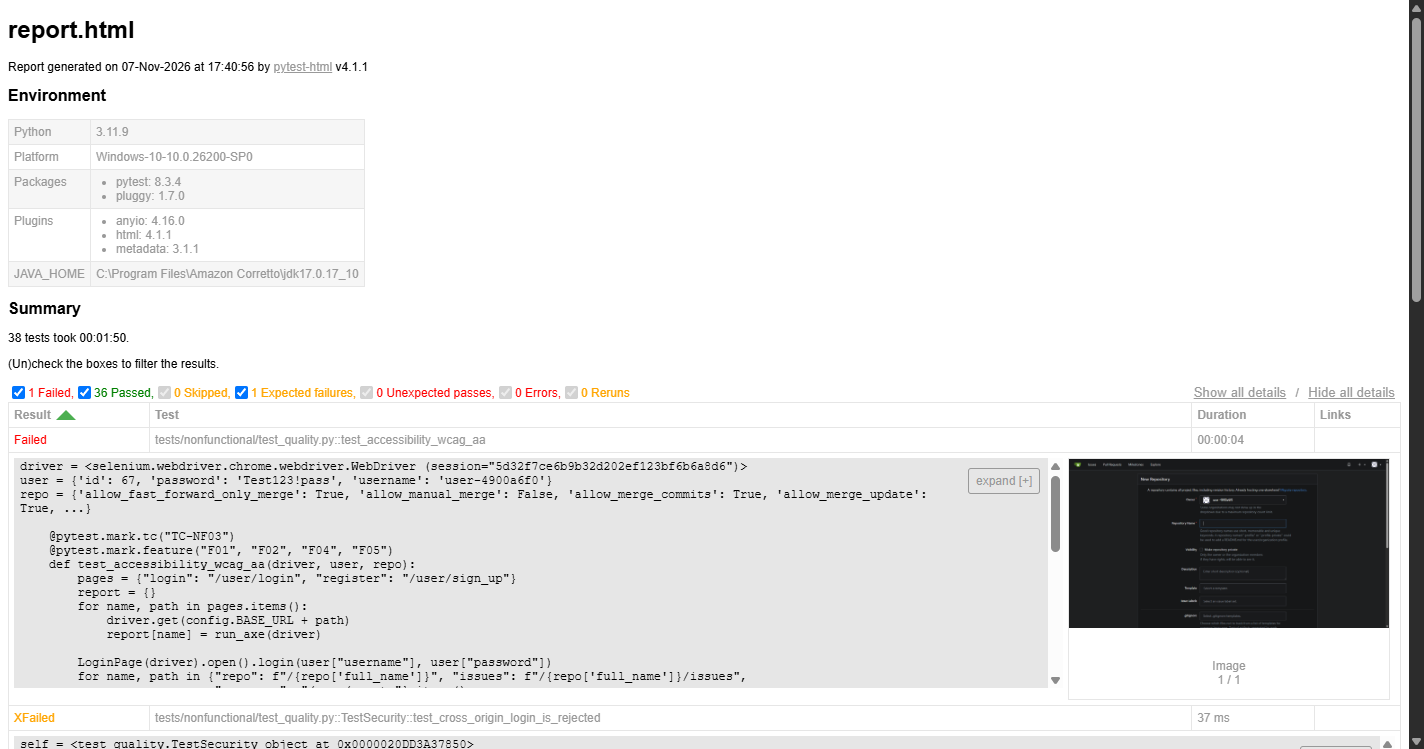
\includegraphics[width=0.85\linewidth]{pytest_html_report.png}
\caption{Raport pytest-html z pełnego przebiegu (38 wykonań).}
\end{figure}

\begin{figure}[H]\centering
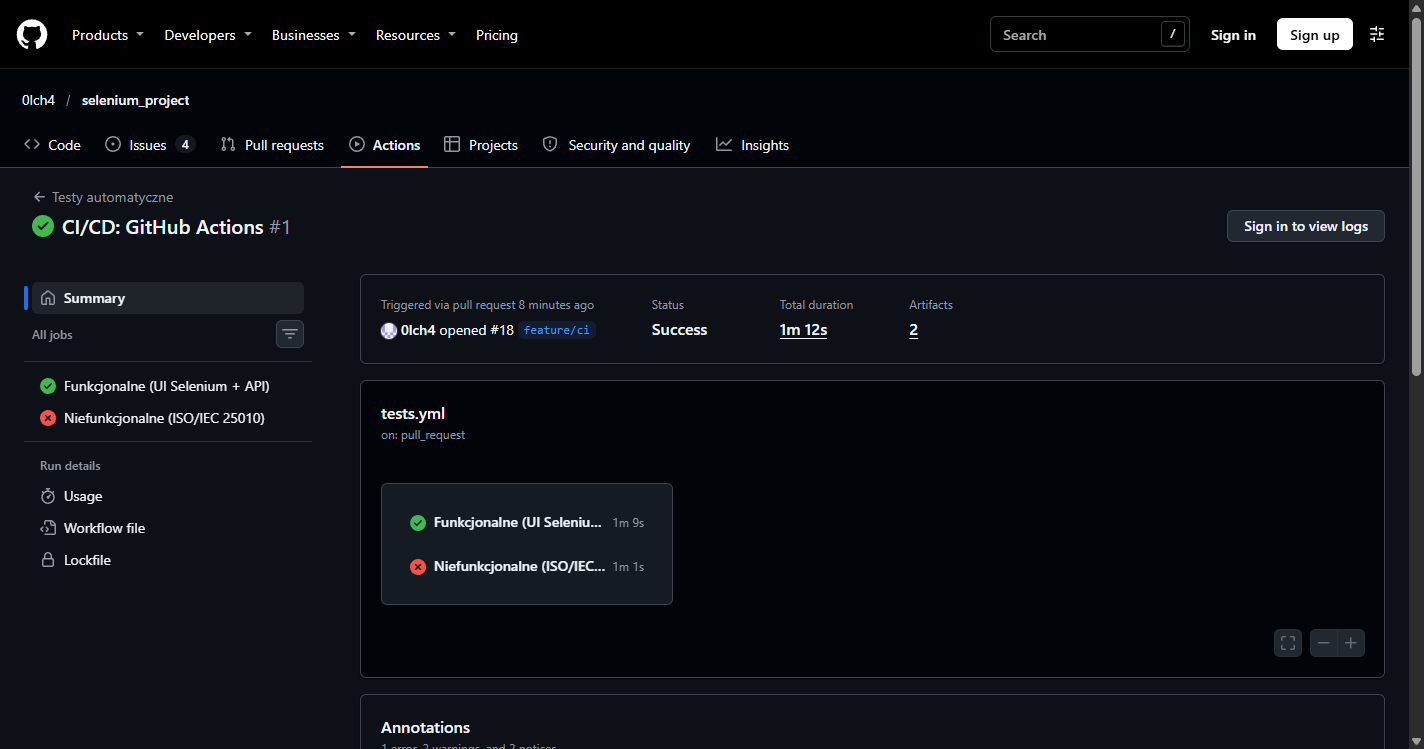
\includegraphics[width=0.85\linewidth]{github_actions_run.png}
\caption{Przebieg GitHub Actions: oba joby zakończone statusem \emph{Success}; znane defekty
DEF-01 i DEF-02 raportowane jako \texttt{xfail}.}
\end{figure}

\begin{figure}[H]\centering
\begin{minipage}{0.49\linewidth}\centering
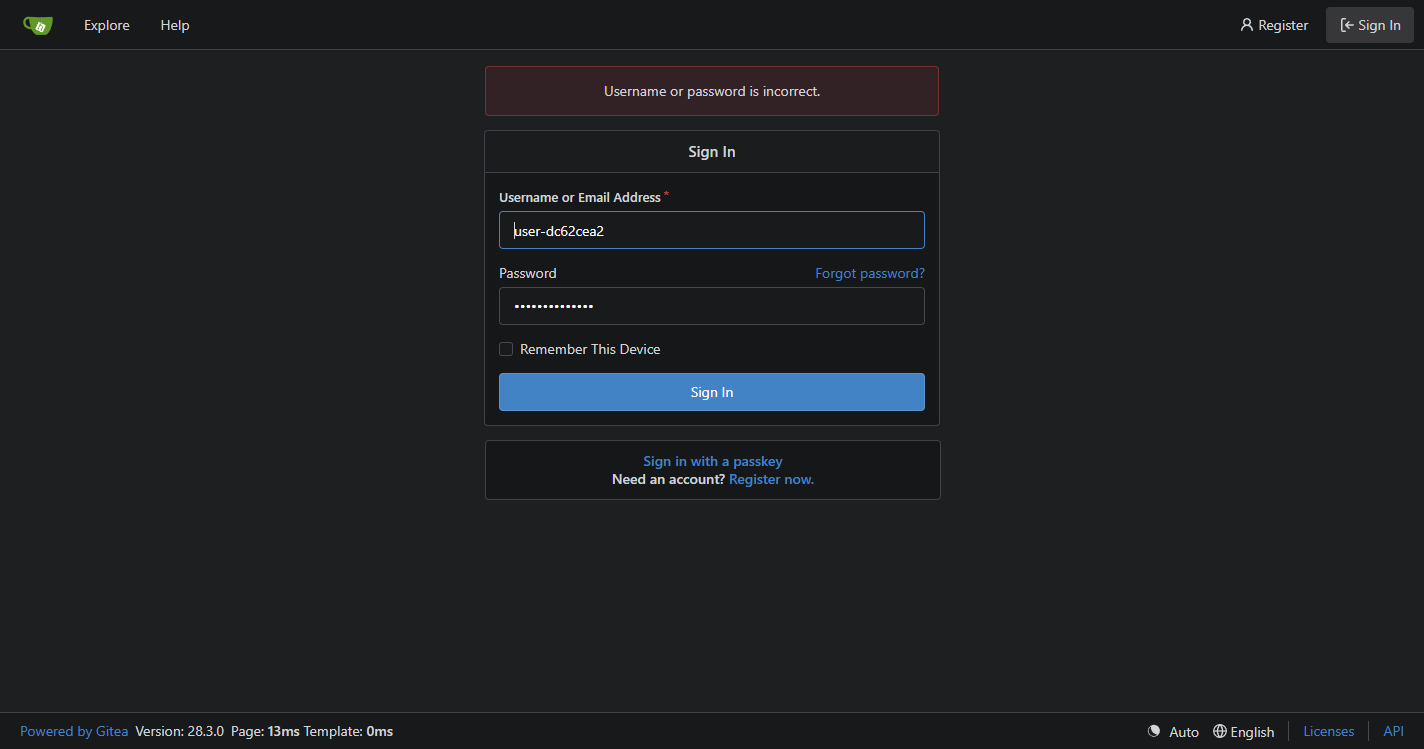
\includegraphics[width=\linewidth]{tc_f04_login_error.png}
\caption{TC-F04: komunikat po błędnym haśle.}
\end{minipage}\hfill
\begin{minipage}{0.49\linewidth}\centering
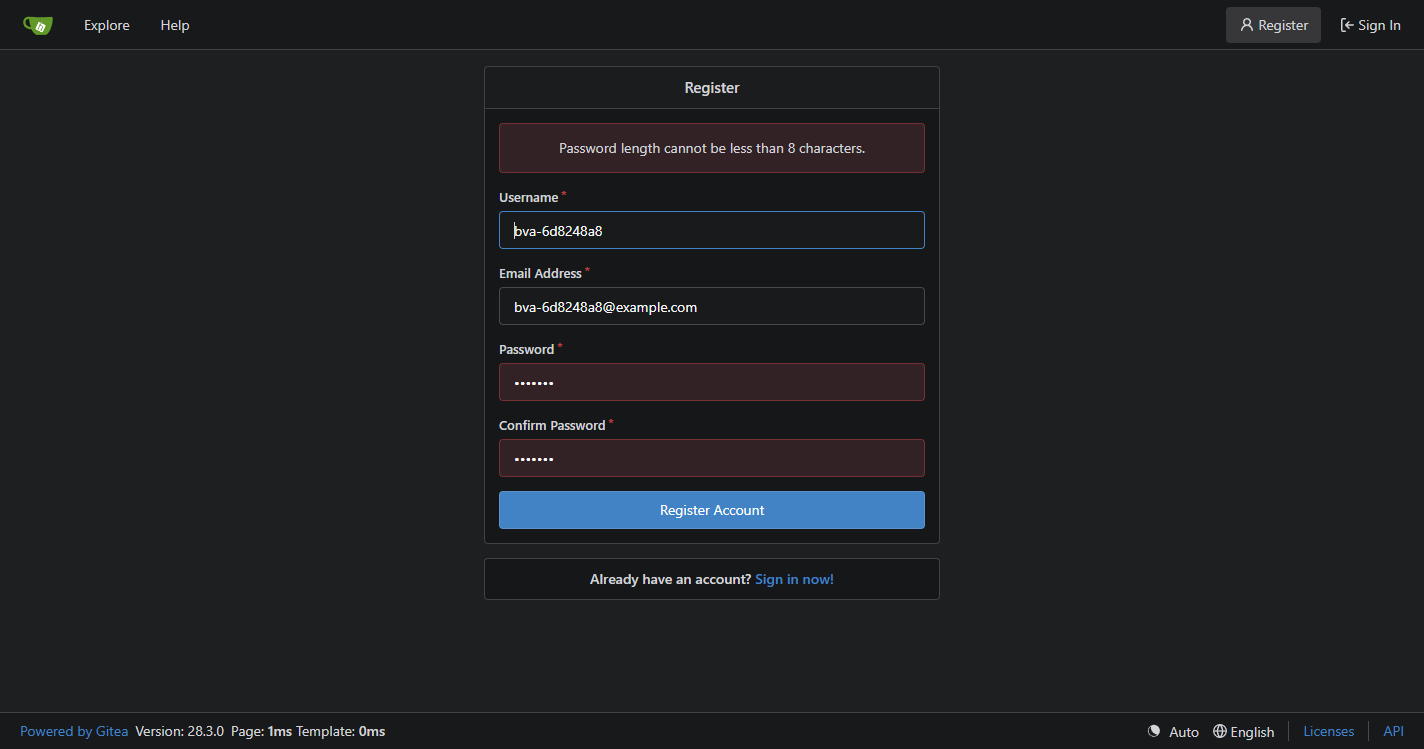
\includegraphics[width=\linewidth]{tc_f02_password_7.png}
\caption{TC-F02: hasło 7-znakowe odrzucone.}
\end{minipage}
\end{figure}

\begin{figure}[H]\centering
\begin{minipage}{0.49\linewidth}\centering
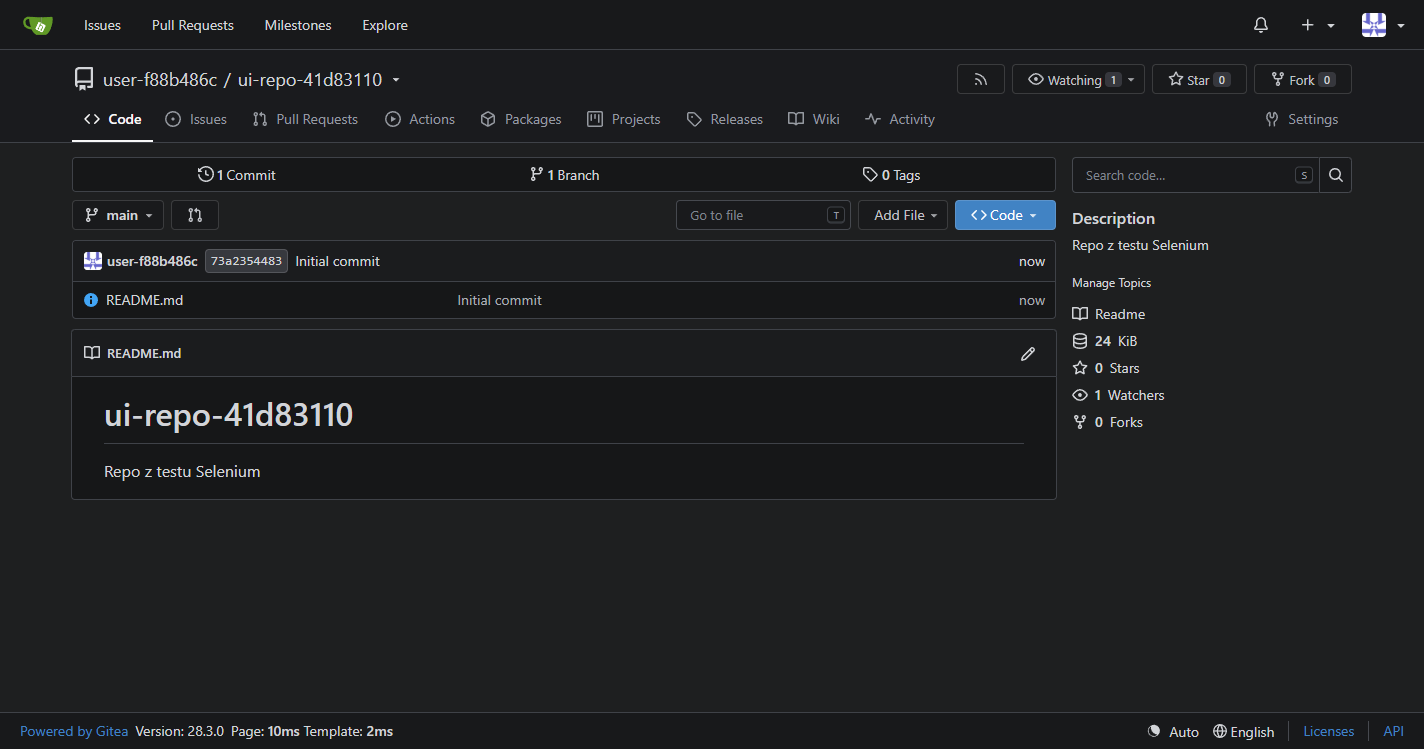
\includegraphics[width=\linewidth]{tc_f05_repo_readme.png}
\caption{TC-F05: repozytorium z README.}
\end{minipage}\hfill
\begin{minipage}{0.49\linewidth}\centering
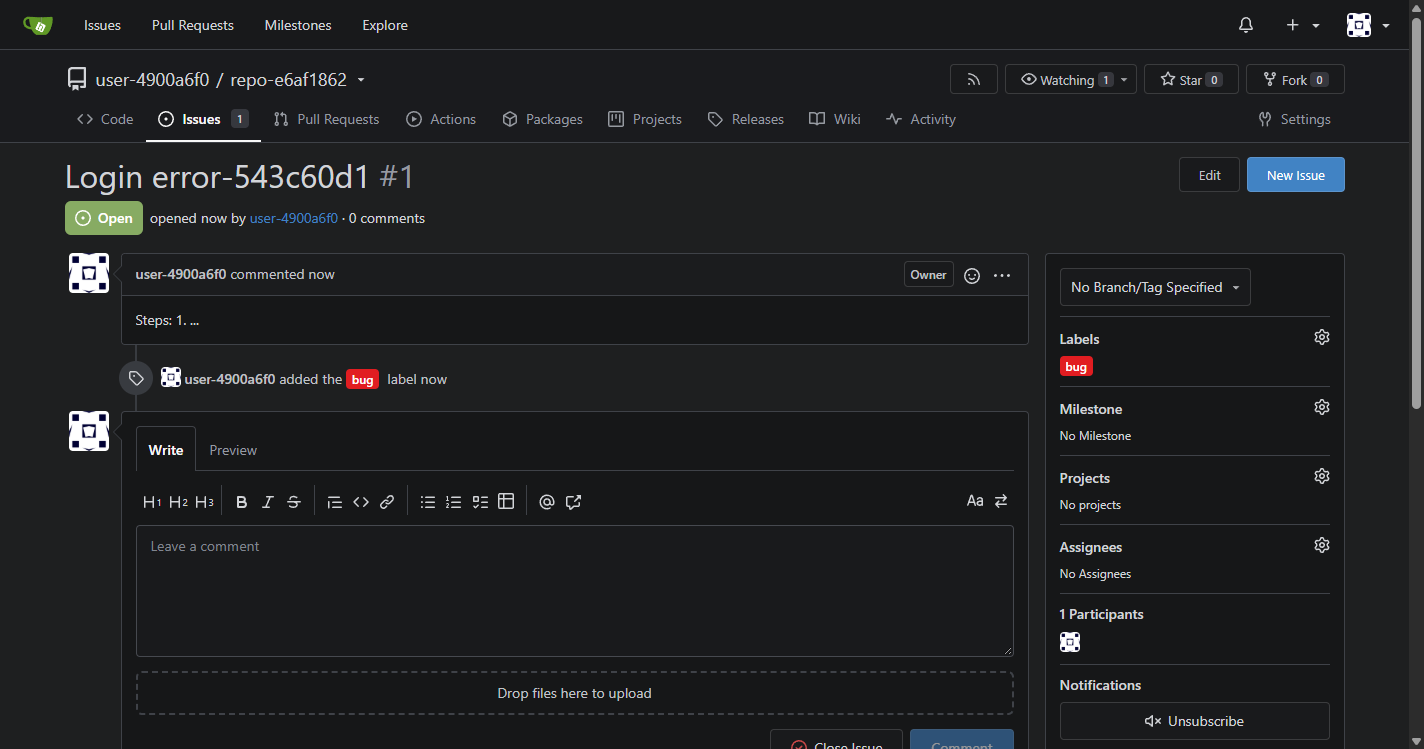
\includegraphics[width=\linewidth]{tc_f07_issue_label.png}
\caption{TC-F07: zgłoszenie z etykietą \texttt{bug}.}
\end{minipage}
\end{figure}

\begin{figure}[H]\centering
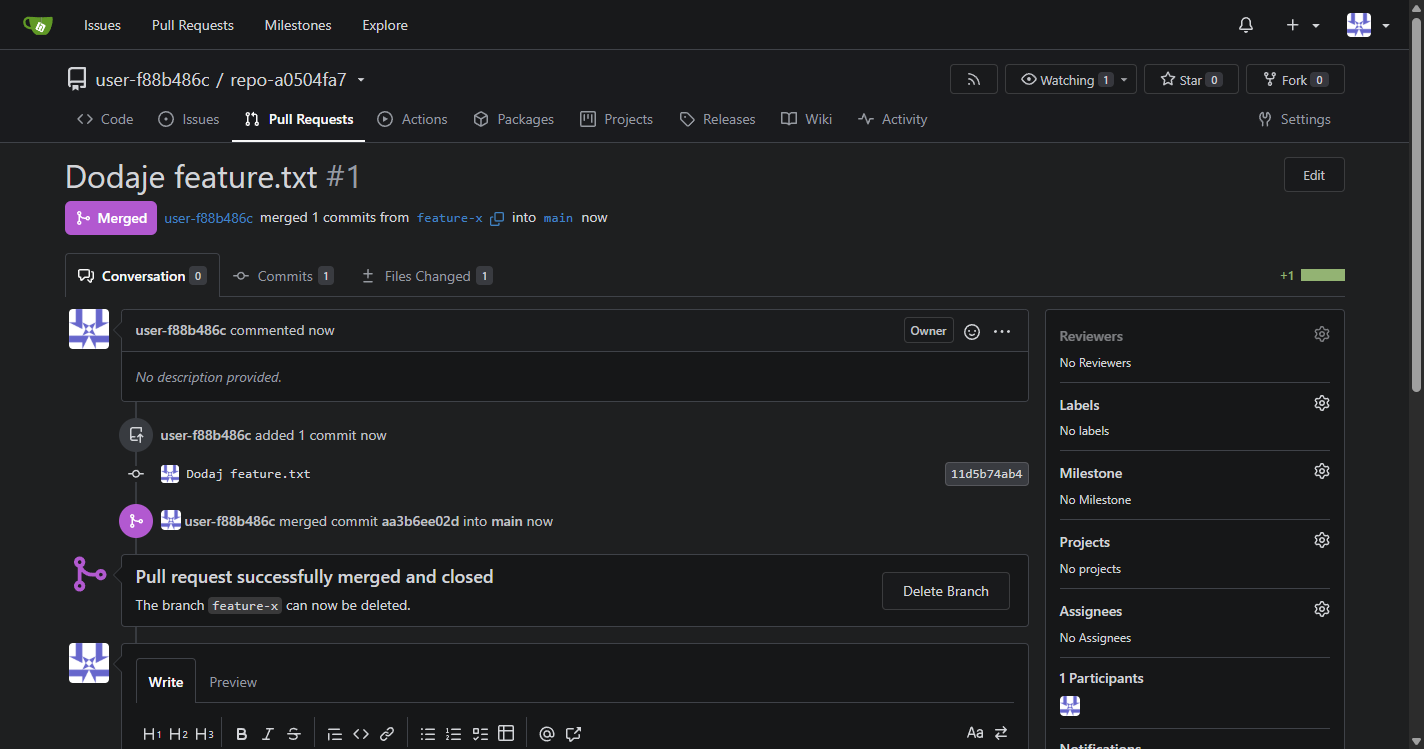
\includegraphics[width=0.7\linewidth]{tc_f10_pr_merged.png}
\caption{TC-F10: scalony pull request.}
\end{figure}

\subsection{Defekty i obserwacje}
{\small
\begin{longtable}{>{\raggedright\arraybackslash}p{\dimexpr 0.090\linewidth-2\tabcolsep\relax}>{\raggedright\arraybackslash}p{\dimexpr 0.450\linewidth-2\tabcolsep\relax}>{\raggedright\arraybackslash}p{\dimexpr 0.130\linewidth-2\tabcolsep\relax}>{\raggedright\arraybackslash}p{\dimexpr 0.100\linewidth-2\tabcolsep\relax}>{\raggedright\arraybackslash}p{\dimexpr 0.100\linewidth-2\tabcolsep\relax}>{\raggedright\arraybackslash}p{\dimexpr 0.130\linewidth-2\tabcolsep\relax}}
\toprule
\textbf{ID} & \textbf{Tytuł} & \textbf{Wykryty przez} & \textbf{Ważność} & \textbf{Priorytet} & \textbf{Status} \\
\midrule
\endhead
DEF-01 & Formularz logowania akceptuje żądania cross-site (login CSRF) & TC-NF04 & Niska & Niski & Otwarty \\
DEF-02 & Krytyczne naruszenia WCAG 2.1 AA na kluczowych widokach & TC-NF03 & Średnia & Średni & Otwarty \\
OBS-01 & Brak nagłówka \texttt{Content-Security-Policy} & TC-NF04 & – & – & Obserwacja \\
OBS-02 & Niewystarczający kontrast tekstu (axe \texttt{color-contrast}, serious) & TC-NF03 & – & – & Obserwacja \\
\bottomrule
\end{longtable}
}
\needspace{8\baselineskip}\subsubsection{DEF-01 – login CSRF}
- \textbf{Kroki:} \texttt{POST /\allowbreak{}user/\allowbreak{}login} z nagłówkami \texttt{Origin: http:/\allowbreak{}/\allowbreak{}evil.example}, \texttt{Sec-Fetch-Site: cross-site} i poprawnymi danymi.

- \textbf{Oczekiwany rezultat:} odrzucenie żądania (403), tak jak dla innych akcji zmieniających stan (\texttt{/\allowbreak{}repo/\allowbreak{}create} zwraca 403).

- \textbf{Rzeczywisty rezultat:} \texttt{303 -> /\allowbreak{}}, ustawiona sesja zalogowanego użytkownika.

- \textbf{Wpływ:} atakujący może zalogować ofiarę na swoje konto (session fixation / login CSRF).

- \textbf{Automatyzacja:} \texttt{tests/\allowbreak{}nonfunctional/\allowbreak{}test\_quality.py::TestSecurity::test\_cross\_origin\_login\_is\_rejected} (\texttt{xfail strict}).

\needspace{8\baselineskip}\subsubsection{DEF-02 – dostępność (axe-core 4.10.2, reguły wcag2a/wcag2aa/wcag21aa)}
{\small
\begin{longtable}{>{\raggedright\arraybackslash}p{\dimexpr 0.333\linewidth-2\tabcolsep\relax}>{\raggedright\arraybackslash}p{\dimexpr 0.333\linewidth-2\tabcolsep\relax}>{\raggedright\arraybackslash}p{\dimexpr 0.333\linewidth-2\tabcolsep\relax}}
\toprule
\textbf{Widok} & \textbf{Krytyczne} & \textbf{Poważne (serious)} \\
\midrule
\endhead
\texttt{/\allowbreak{}user/\allowbreak{}login} & aria-required-children (2) & color-contrast (4) \\
\texttt{/\allowbreak{}user/\allowbreak{}sign\_up} & aria-required-children (2) & color-contrast (4) \\
\texttt{/\allowbreak{}\{owner\}/\allowbreak{}\{repo\}} & aria-required-children (3), button-name (1) & aria-prohibited-attr, color-contrast, link-name \\
\texttt{/\allowbreak{}\{owner\}/\allowbreak{}\{repo\}/\allowbreak{}issues} & aria-required-children (4) & aria-prohibited-attr, color-contrast (8) \\
\texttt{/\allowbreak{}repo/\allowbreak{}create} & aria-required-children (2), label (4) & aria-input-field-name (3), color-contrast, link-in-text-block \\
\bottomrule
\end{longtable}
}
- \textbf{Oczekiwany rezultat (kryterium TC-NF03):} brak naruszeń o wpływie \texttt{critical}.

- \textbf{Wpływ:} użytkownicy czytników ekranu nie otrzymują poprawnej struktury menu (role \texttt{menu} bez wymaganych dzieci), pola formularza nowego repo bez etykiet, przycisk bez nazwy dostępnej.

- Pełne dane: \texttt{reports/\allowbreak{}axe.json} (generowany przy każdym przebiegu).



% ------------------------------------------------------------------ 7
\section{Wyniki LLM-as-a-Judge}

\subsection{Architektura}
Rozwiązanie jest powtarzalnym potokiem złożonym z dwóch etapów:
\begin{enumerate}
  \item \textbf{Capture} (\texttt{llm\_judge/capture.py}) -- przez API tworzony jest stały zestaw
        danych demonstracyjnych (użytkownik, repozytorium ze strukturą plików, 5 zgłoszeń z etykietami),
        następnie Selenium wykonuje zrzuty 4 widoków w stałej rozdzielczości 1440$\times$900 i zapisuje
        kontekst każdego widoku (URL, cel, typowe zadanie użytkownika) do \texttt{views.json}.
  \item \textbf{Judge} (\texttt{llm\_judge/judge.py}) -- dla każdego widoku model językowy otrzymuje
        \emph{prompt systemowy z rubryką} (osobny plik \texttt{llm\_judge/prompts/judge\_rubric.md}),
        zrzut ekranu i kontekst; odpowiedź jest wymuszona schematem JSON i walidowana modelem
        \texttt{pydantic} (dokładnie 8 wymiarów, ocena całkowita 1--5, dowód i uzasadnienie);
        każdy widok oceniany jest w \textbf{3 niezależnych przebiegach}, a wynik agregowany medianą
        z miarą rozrzutu (max -- min).
\end{enumerate}

Zaimplementowano dwa wymienne \textbf{backendy} wywołania modelu (wybór \texttt{--backend},
domyślnie \texttt{auto}):
\begin{itemize}
  \item \texttt{api} -- Anthropic SDK (\texttt{client.beta.messages.parse}) z obrazem w bloku
        \texttt{image} (base64), \emph{structured outputs} na podstawie klasy pydantic, cache'owanym
        promptem systemowym i serwerowym mechanizmem \emph{fallback} przy odmowie modelu;
        wymaga klucza \texttt{ANTHROPIC\_API\_KEY} (plik \texttt{.env}),
  \item \texttt{cli} -- bezgłowe wywołanie Claude Code (\texttt{claude -p --output-format json
        --json-schema ... --tools Read}); model odczytuje plik PNG narzędziem \texttt{Read},
        a wynik jest ograniczony tym samym schematem JSON i walidowany tym samym modelem pydantic.
\end{itemize}
W obu przypadkach sędzią jest ten sam model (\texttt{claude-opus-5-5}). Werdykt widoku:
\textbf{PASS}, gdy średnia z median $\geq 3{,}5$ i żaden wymiar nie ma mediany $< 2$.

\subsection{Rubryka oceny i skala}
Rubryka obejmuje 8 wymiarów opartych o \textbf{heurystyki użyteczności Nielsena} (H1--H10)
oraz kryteria sukcesu \textbf{WCAG 2.2}; prompt i wyniki są w języku angielskim.

\begin{longtable}{p{0.2\linewidth}p{0.2\linewidth}p{0.52\linewidth}}
\toprule \textbf{Wymiar (id)} & \textbf{Podstawa} & \textbf{Co oceniano} \\ \midrule \endhead
\texttt{visual\_hierarchy} & Gestalt, wzorzec F & dominacja głównej akcji, grupowanie, wyrównanie, odstępy \\
\texttt{consistency} & Nielsen H4 & spójność komponentów, ikon, kolorów i nazewnictwa z konwencjami platform Git \\
\texttt{system\_status} & Nielsen H1 & widoczność położenia użytkownika i stanu obiektów (open/closed, liczniki) \\
\texttt{language\_clarity} & Nielsen H2, WCAG 3.3.2 & zrozumiałość etykiet, przycisków, komunikatów \\
\texttt{error\_prevention} & Nielsen H5, H9 & oznaczenie pól wymaganych, podpowiedzi, ostrożność przy akcjach nieodwracalnych \\
\texttt{efficiency} & Nielsen H6, H7 & liczba kroków, skróty i filtry, rozpoznawanie zamiast przypominania \\
\texttt{minimalism} & Nielsen H8 & brak zbędnych elementów, adekwatna gęstość informacji \\
\texttt{accessibility} & WCAG 1.4.3, 1.4.11, 2.4.7, 2.5.8 & kontrast, rozmiar celów, czytelność, nieopieranie się na kolorze \\
\bottomrule
\end{longtable}

\begin{longtable}{p{0.15\linewidth}p{0.77\linewidth}}
\toprule \textbf{Ocena} & \textbf{Kotwica} \\ \midrule \endhead
5 -- wzorcowo & brak uwag; przykład dobrej praktyki \\
4 -- dobrze & drobne niedociągnięcia kosmetyczne, bez wpływu na zadanie \\
3 -- akceptowalnie & zauważalne problemy spowalniające część użytkowników; zadanie wykonalne \\
2 -- słabo & poważne problemy; użytkownik prawdopodobnie popełni błąd \\
1 -- krytycznie & problem blokujący zadanie lub wykluczający grupę użytkowników \\
\bottomrule
\end{longtable}

Reguły w prompcie ograniczają typowe błędy sędziów LLM: każda ocena musi mieć dowód widoczny na
zrzucie, ocena $\leq 3$ wymaga wskazania problemu i rekomendacji, zakaz zawyżania ocen i ocenianie
wymiarów niezależnie (przeciwdziałanie efektowi aureoli).

\subsection{Oceniane widoki}
\begin{figure}[H]\centering
\begin{minipage}{0.49\linewidth}\centering
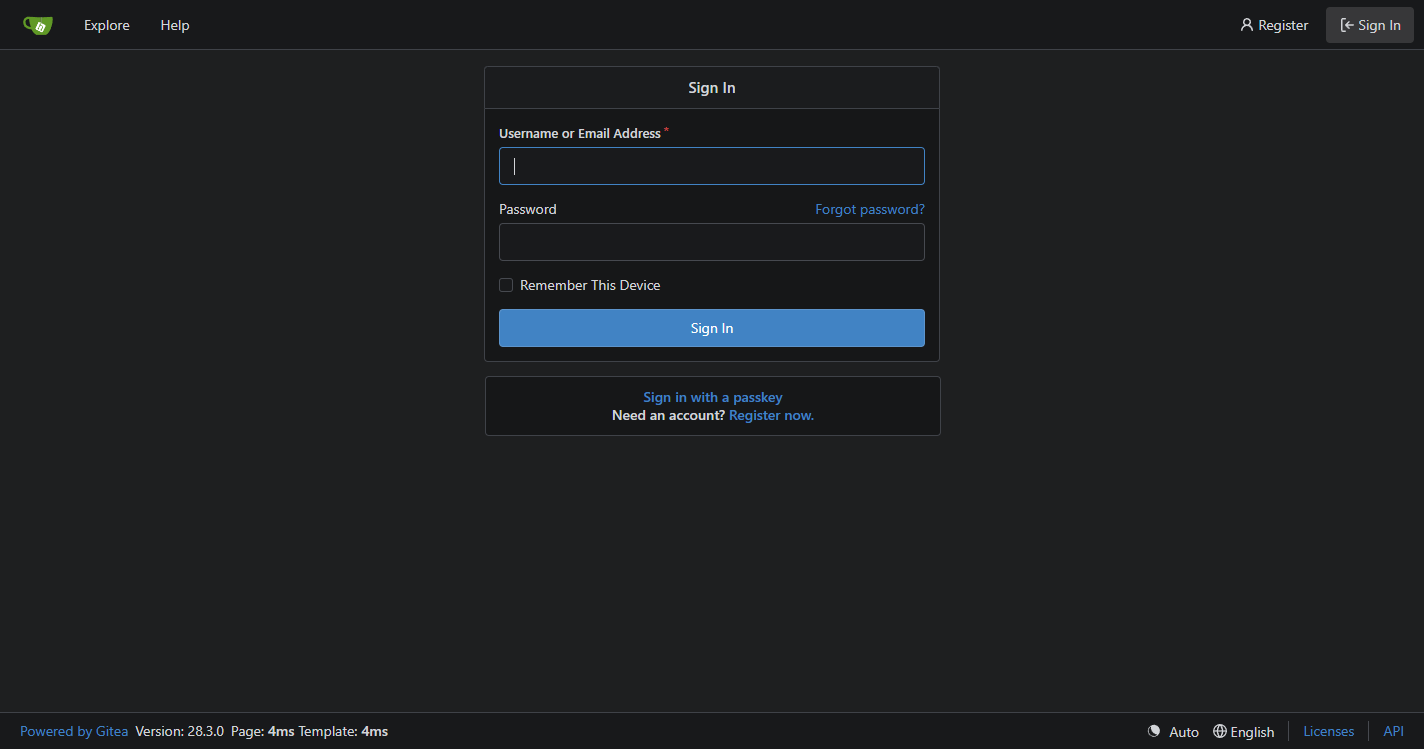
\includegraphics[width=\linewidth]{login.png}
\caption{\texttt{login} -- logowanie.}
\end{minipage}\hfill
\begin{minipage}{0.49\linewidth}\centering
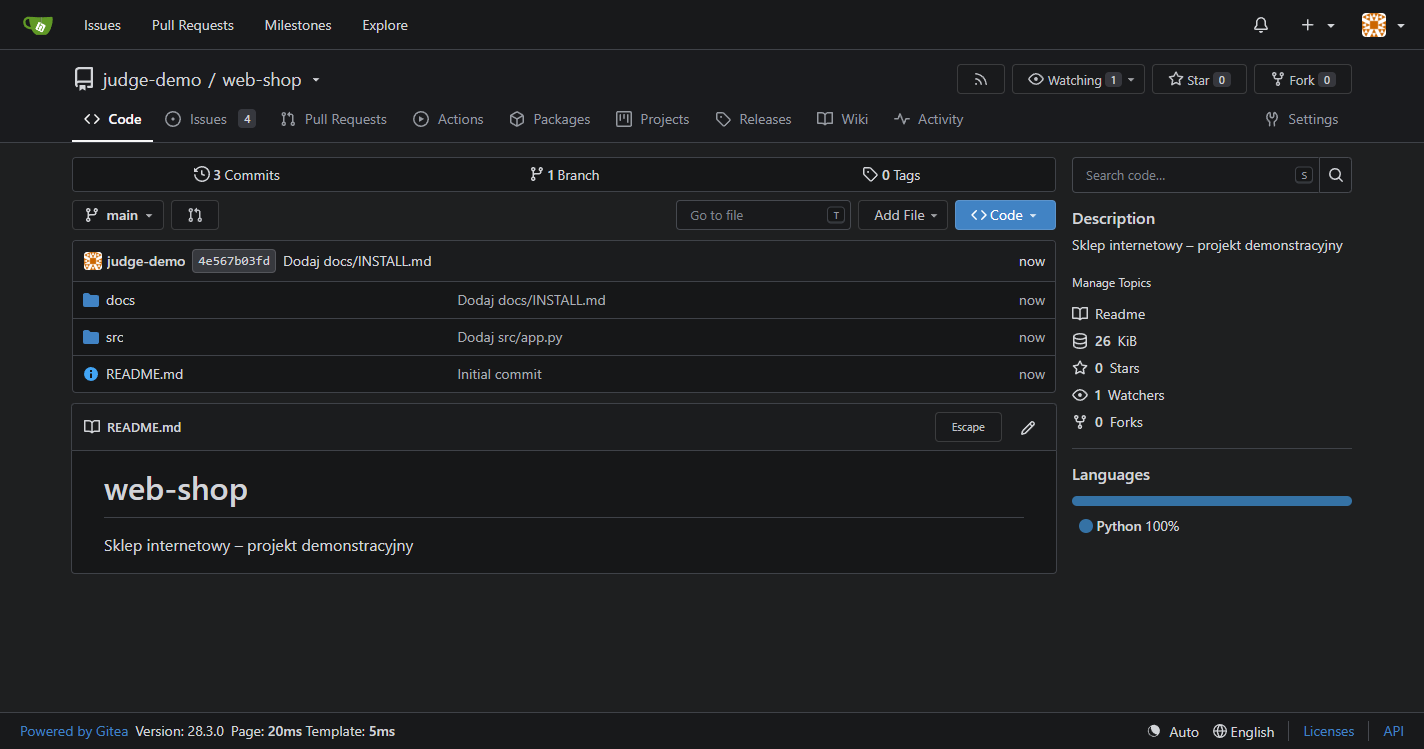
\includegraphics[width=\linewidth]{repo_home.png}
\caption{\texttt{repo\_home} -- strona repozytorium.}
\end{minipage}
\end{figure}
\begin{figure}[H]\centering
\begin{minipage}{0.49\linewidth}\centering
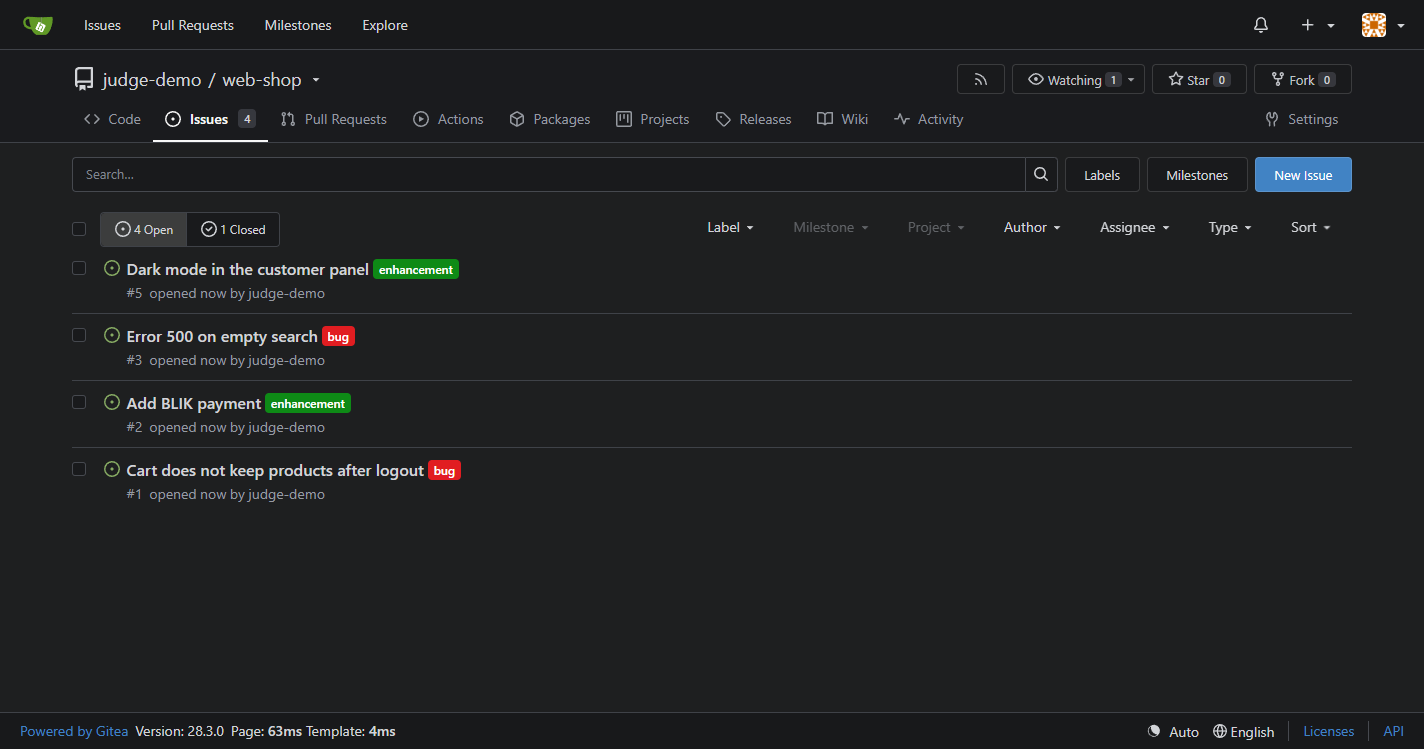
\includegraphics[width=\linewidth]{issues_list.png}
\caption{\texttt{issues\_list} -- lista zgłoszeń.}
\end{minipage}\hfill
\begin{minipage}{0.49\linewidth}\centering
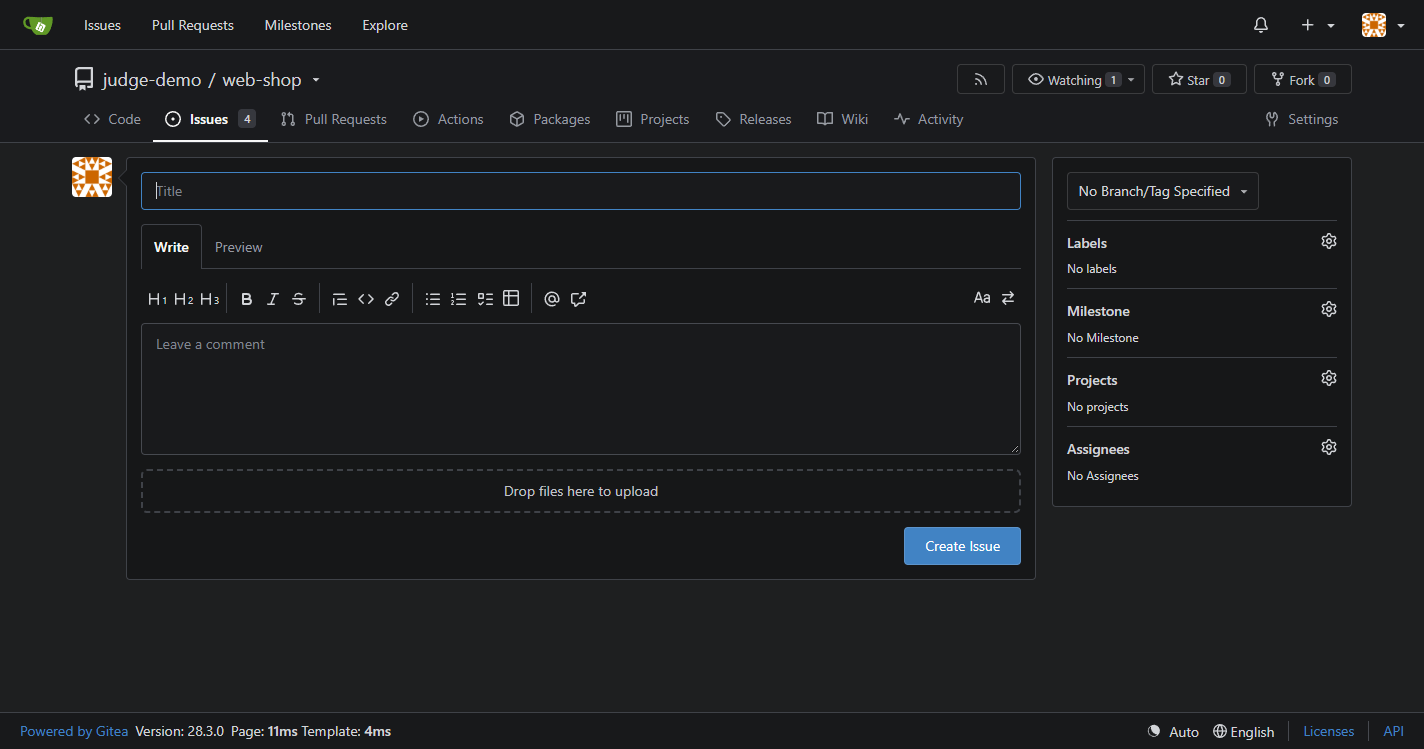
\includegraphics[width=\linewidth]{new_issue.png}
\caption{\texttt{new\_issue} -- formularz nowego zgłoszenia.}
\end{minipage}
\end{figure}

\subsection{Wyniki i werdykt}
Backend \texttt{cli}, model \texttt{claude-opus-5-5}, 3 przebiegi na widok. Komórki: mediana ($\pm$ rozrzut = max $-$ min z przebiegów).

{\small
\begin{longtable}{p{\dimexpr 0.200\linewidth-2\tabcolsep\relax}p{\dimexpr 0.200\linewidth-2\tabcolsep\relax}p{\dimexpr 0.200\linewidth-2\tabcolsep\relax}p{\dimexpr 0.200\linewidth-2\tabcolsep\relax}p{\dimexpr 0.200\linewidth-2\tabcolsep\relax}}
\toprule
\textbf{Wymiar} & \textbf{login} & \textbf{repo\_home} & \textbf{issues\_list} & \textbf{new\_issue} \\
\midrule
\endhead
\texttt{visual\_hierarchy} & 4 ($\pm$0) & 4 ($\pm$0) & 4 ($\pm$0) & 4 ($\pm$0) \\
\texttt{consistency} & 3 ($\pm$1) & 4 ($\pm$1) & 5 ($\pm$0) & 5 ($\pm$0) \\
\texttt{system\_status} & 4 ($\pm$0) & 4 ($\pm$0) & 4 ($\pm$0) & 4 ($\pm$0) \\
\texttt{language\_clarity} & 4 ($\pm$1) & 3 ($\pm$0) & 4 ($\pm$0) & 3 ($\pm$1) \\
\texttt{error\_prevention} & 3 ($\pm$0) & 4 ($\pm$0) & 4 ($\pm$0) & 3 ($\pm$0) \\
\texttt{efficiency} & 5 ($\pm$1) & 5 ($\pm$0) & 4 ($\pm$1) & 4 ($\pm$1) \\
\texttt{minimalism} & 4 ($\pm$0) & 4 ($\pm$0) & 4 ($\pm$0) & 4 ($\pm$0) \\
\texttt{accessibility} & 3 ($\pm$0) & 3 ($\pm$0) & 3 ($\pm$0) & 3 ($\pm$0) \\
\textbf{średnia median} & \textbf{3.75} & \textbf{3.88} & \textbf{4} & \textbf{3.75} \\
\textbf{werdykt} & \textbf{PASS} & \textbf{PASS} & \textbf{PASS} & \textbf{PASS} \\
\bottomrule
\end{longtable}
}
{\renewcommand{\arraystretch}{1.2}
{\small
\begin{longtable}{p{\dimexpr 0.150\linewidth-2\tabcolsep\relax}p{\dimexpr 0.200\linewidth-2\tabcolsep\relax}p{\dimexpr 0.650\linewidth-2\tabcolsep\relax}}
\toprule
\textbf{Widok} & \textbf{Wymiar} & \textbf{Rekomendacja (wysoki priorytet, przebieg 1)} \\
\midrule
\endhead
login & \texttt{consistency} & Mark the Password field as required with the same red asterisk as the username field, or add a note that all fields are required. \\
issues\_list & \texttt{accessibility} & Raise the contrast of the metadata text, disabled filters and label pills (for example, darken the green 'enhancement' background or use dark text) to reach at least 4.5:1. Enlarge row checkboxes and their click areas to at least 24$\times$24 px. \\
new\_issue & \texttt{error\_prevention} & Mark the Title field as required (for example a visible label 'Title *'). Disable the 'Create Issue' button, or show a validation message inline, while the title is empty. \\
new\_issue & \texttt{language\_clarity} & Change the body placeholder from 'Leave a comment' to 'Describe the issue (Markdown supported)'. Add persistent visible labels above the Title and Description fields. \\
\bottomrule
\end{longtable}
}}


\textbf{Interpretacja.} Wszystkie 4 widoki otrzymały werdykt \textbf{PASS} (średnie median
3,62--4,12; najniżej formularz nowego zgłoszenia, najwyżej lista zgłoszeń); żaden wymiar nie
spadł poniżej 3. Najsłabszym wymiarem jest \texttt{accessibility}
-- mediana 3 na każdym widoku, przy zerowym rozrzucie między przebiegami. Sędzia wskazywał
niski kontrast tekstu drugorzędnego w motywie ciemnym oraz zbyt małe cele klikalne
(np.~pola wyboru wierszy), co jest zgodne z wynikiem obiektywnego testu TC-NF03
(axe-core: \texttt{color-contrast}, DEF-02/OBS-02). Drugi powtarzający się obszar to
\texttt{error\_prevention} i \texttt{language\_clarity} w formularzach: brak oznaczenia
wymaganego pola tytułu i mylący placeholder ,,Leave a comment'' w formularzu nowego zgłoszenia
oraz niespójne oznaczenie pól wymaganych na stronie logowania. Najwyżej oceniono
\texttt{consistency} i \texttt{minimalism} (konwencje znane z platform Git, liczniki, filtry).
Rozrzut ocen wynosił co najwyżej 1 punkt, a w 22 z 32 komórek był zerowy, co wskazuje na
dobrą powtarzalność sędziego przy wymuszonym schemacie odpowiedzi; największą zmienność
(5 wymiarów z rozrzutem 1) miał formularz nowego zgłoszenia.

\textbf{Rekomendacje UI/UX} (zbiorczo): zwiększyć kontrast tekstu pomocniczego i obramowań pól
do co najmniej 4,5:1 / 3:1, powiększyć cele klikalne do 24$\times$24~px, oznaczyć pola wymagane
i walidować je inline, zastąpić ogólne placeholdery opisowymi etykietami, ukryć metryki
renderowania w stopce przed niezalogowanymi użytkownikami.

\subsection{Ograniczenia}
Sędzia LLM nie zastępuje testów z udziałem użytkowników: ocenia statyczny zrzut (bez interakcji,
stanów hover i fokusu), a jego oceny nie zostały skalibrowane względem ocen ekspertów.
Powtarzalność ograniczono przez stały zestaw danych i rozdzielczość, wymuszony schemat odpowiedzi
oraz agregację 3 przebiegów; rozrzut ocen raportowany jest jawnie. Wyniki LLM-as-a-Judge są spójne
z obiektywnym testem TC-NF03 (axe-core) -- oba wskazują obszar dostępności jako najsłabszy.

% ------------------------------------------------------------------ 8
\section{Podsumowanie i wnioski}

\subsection{Podsumowanie}
Zaprojektowano 22 przypadki testowe (17 funkcjonalnych, 5 niefunkcjonalnych) i wszystkie
zautomatyzowano; 12 przypadków wykorzystuje Selenium WebDriver. Wykonano 38 testów
(parametryzacja): 36 zaliczonych i 2 oczekiwane niepowodzenia (\texttt{xfail}) odpowiadające
potwierdzonym defektom: TC-NF03 (DEF-02) i jedna kontrola TC-NF04 (DEF-01). Pełny przebieg trwa około 110~s, a pipeline CI uruchamia testy przy każdym pull requeście.

\subsection{Pokrycie}
\begin{itemize}
  \item pokrycie funkcji: 11 z 14 (79\%); \emph{Must} 7/7, \emph{Should} 3/3, \emph{Could} 1/3,
        \emph{Won't} 0/1 (poza zakresem),
  \item pokrycie tablicy decyzyjnej TC-F14: 6/6 reguł (100\%); wartości brzegowe TC-F02: 2/2,
  \item charakterystyki ISO/IEC 25010: wydajność, bezpieczeństwo, zdolność do interakcji,
        kompatybilność (4 z 9).
\end{itemize}

\subsection{Ocena kryteriów wyjścia}
Wszystkie przypadki zostały wykonane, wszystkie przypadki o priorytecie wysokim zaliczono.
Wykryte defekty dotyczą dostępności (średnia ważność) i login CSRF (niska), więc nie ma otwartych
defektów krytycznych w funkcjach \emph{Must}. Kryteria wyjścia uznano za spełnione, a defekty
DEF-01 i DEF-02 zarejestrowano jako znane ryzyko do zgłoszenia twórcom Gitei.

\subsection{Rekomendacje}
\begin{itemize}
  \item poprawić role ARIA menu (\texttt{aria-required-children}) i etykiety pól formularza
        nowego repozytorium (DEF-02) oraz kontrast tekstu pomocniczego (OBS-02),
  \item objąć formularz logowania tą samą ochroną cross-origin co pozostałe akcje (DEF-01),
  \item rozważyć nagłówek \texttt{Content-Security-Policy} (OBS-01),
  \item rozszerzyć zakres o organizacje i wiki (ryzyko rezydualne) oraz testy obciążeniowe
        operacji zapisu i większej liczby użytkowników.
\end{itemize}

\subsection{Napotkane trudności}
\begin{itemize}
  \item Gitea 28 zrezygnowała z tokenu \texttt{\_csrf} w formularzach na rzecz weryfikacji
        nagłówków \texttt{Origin} i \texttt{Sec-Fetch-Site} -- wymagało to dostosowania klienta HTTP
        i zainspirowało przypadki bezpieczeństwa w TC-NF04,
  \item formularz scalania PR jest renderowany przez Vue, a wiele akcji wysyła \texttt{fetch}
        i przeładowuje stronę -- prowadziło to do niestabilnego testu TC-F08
        (\texttt{StaleElementReferenceException}); naprawiono to w warstwie Page Object,
  \item Selenium 4.27 nie pobierał sterownika Edge (wycofany adres serwera) -- rozwiązane aktualizacją do 4.50,
  \item brak lokalnej instalacji LaTeX -- PDF raportu kompilowany jest w GitHub Actions.
\end{itemize}

\end{document}
